%============================================================================
% tento soubor pouzijte jako zaklad
% (c) 2008 Michal Bidlo
% E-mail: bidlom AT fit vutbr cz
%============================================================================
% kodovaní: utf-8 (zmena prikazem iconv, recode nebo cstocs)
%----------------------------------------------------------------------------
% zpracování: make, make pdf, make desky, make clean
% připomínky posílejte na e-mail: bidlom AT fit.vutbr.cz
% vim: set syntax=tex encoding=utf-8:
%============================================================================
\documentclass[english,cover]{fitthesis} % odevzdani do wisu - odkazy, na ktere se da klikat
%\documentclass[cover,print]{fitthesis} % pro tisk - na odkazy se neda klikat
%\documentclass[english,print]{fitthesis} % pro tisk - na odkazy se neda klikat
%      \documentclass[english]{fitthesis}
% * Je-li prace psana v anglickem jazyce, je zapotrebi u tridy pouzit 
%   parametr english nasledovne:
%      \documentclass[english]{fitthesis}
% * Neprejete-li si vysazet na prvni strane dokumentu desky, zruste 
%   parametr cover

% zde zvolime kodovani, ve kterem je napsan text prace
% "latin2" pro iso8859-2 nebo "cp1250" pro windows-1250, "utf8" pro "utf-8"
%\usepackage{ucs}
\usepackage[utf8]{inputenc}
\usepackage[T1, IL2]{fontenc}
\usepackage{url}
\DeclareUrlCommand\url{\def\UrlLeft{<}\def\UrlRight{>} \urlstyle{tt}}

%zde muzeme vlozit vlastni balicky
\usepackage{amsmath}
\usepackage{amsthm}
\usepackage{color}
\usepackage{comment}
\usepackage{graphicx}
\usepackage{caption}
\usepackage{subcaption}
\usepackage{multirow}
\usepackage{changepage}
\newtheorem{math_def}{Definition}[chapter] % 3. parametr zajisti cislovani "<sekce>.<číslo definice>"
\newcommand{\term}[1]{\emph{#1}}           % novy termin v textu prace
\newcommand{\srccode}[1]{{\tt #1}}         % fragment zdrojaku v textu
\newcommand{\vars}[1]{{\bold{#1}}}         % matematicke vyrazy - mnozina promennych
\newcommand{\ignore}[1]{}                  % komentar v radku
\newcommand{\todo}[1]{{\color{red}#1}}
\newcommand{\uncertain}[1]{{\color{magenta}#1}}
\newcommand{\note}[1]{{\color{green}#1}}

% SP komentar co se hodi zohlednit ve finalni diplomce


% =======================================================================
% balíček "hyperref" vytváří klikací odkazy v pdf, pokud tedy použijeme pdflatex
% problém je, že balíček hyperref musí být uveden jako poslední, takže nemůže
% být v šabloně
\ifWis
\ifx\pdfoutput\undefined % nejedeme pod pdflatexem
\else
  \usepackage{color}
  \usepackage[unicode,colorlinks,hyperindex,plainpages=false,pdftex]{hyperref}
  \definecolor{links}{rgb}{0.4,0.5,0}
  \definecolor{anchors}{rgb}{1,0,0}
  \def\AnchorColor{anchors}
  \def\LinkColor{links}
  \def\pdfBorderAttrs{/Border [0 0 0] }  % bez okrajů kolem odkazů
  \pdfcompresslevel=9
\fi
\fi

% Informace o praci/projektu
%---------------------------------------------------------------------------
\projectinfo{
  % Prace
  project=DP,            % typ prace BP/SP/DP/DR
  year=2013,             % rok
  date=\today,           % datum odevzdani
  % Nazev prace
  title.cs={Aplikace Bayesovských sítí},     % nazev prace v cestine
  title.en={Bayesian Networks Applications}, % nazev prace v anglictine
  % Autor
  author={David Chaloupka},   % jmeno prijmeni autora
  author.title.p=Bc.,         % titul pred jmenem (nepovinne)
  %author.title.a=PhD,        % titul za jmenem (nepovinne)
  % Ustav
  department=UITS, % doplnte prislusnou zkratku: UPSY/UIFS/UITS/UPGM
  % Skolitel
  supervisor=František V. Zbořil, % jmeno prijmeni skolitele
  supervisor.title.p=doc.~Ing.,   % titul pred jmenem (nepovinne)
  supervisor.title.a={CSc.},      % titul za jmenem (nepovinne)
  %Klicova slova, abstrakty, prohlaseni a podekovani je mozne definovat 
  %bud pomoci nasledujicich parametru nebo pomoci vyhrazenych maker (viz dale)
  %===========================================================================
  %Klicova slova
  keywords.cs={Bayesovská síť, pravděpodobnost, inference, učení struktury.}, %klicova slova v ceskem jazyce
  keywords.en={Bayesian network, probability, inference, structure learning.}, %klicova slova v anglickem jazyce
  %Abstract
  abstract.cs={Tato diplomová práce se zabývá možnými aplikacemi Bayesovských sítí. Nejprve se zaměřuje na obecnou teorii pravděpodobnosti, později na úrovni matematiky vysvětluje samotnou teorii Bayesovských sítí, přístupy k inferenci a k učení včetně pochopení silných a~slabých stránek daných technik. V praktické části je kladen důraz na aplikace vyžadující učení Bayesovské sítě, jednak ve smyslu učení parametrů a jednak ve smyslu struktury.}, % abstrakt v ceskem jazyce
  abstract.en={This master's thesis deals with possible applications of Bayesian networks. The theoretical part is mainly of mathematical nature. At first, we focus on general probability theory and later we move on to the theory of Bayesian networks and discuss approaches to inference and to model learning while providing an explanation of pros and cons of these techniques. The practical part focuses on applications suitable for learning a Bayesian network, both in terms of network parameters as well as structure.}, % abstrakt v anglickem jazyce
  %Prohlaseni
  declaration={Prohlašuji, že jsem tuto diplomovou práci vypracoval samostatně pod vedením pana doc.~Ing. Františka V. Zbořila, CSc.},
  %Podekovani (nepovinne)
  acknowledgment={Na tomto místě bych rád poděkoval svému vedoucímu, docentu Františku V. Zbořilovi, za cenné rady, odborné vedení a vstřícný přístup v nesnázích při řešení této práce.} % nepovinne
}


\begin{document}
  % Vysazeni titulnich stran
  % ----------------------------------------------
  \maketitle
  % Obsah
  % ----------------------------------------------
  \tableofcontents
  
  % Seznam obrazku a tabulek (pokud prace obsahuje velke mnozstvi obrazku, tak se to hodi)
  % \listoffigures
  % \listoftables 

  % Text prace
  % ----------------------------------------------

  








%end-of-inserted-header
%=========================================================================
% (c) Michal Bidlo, Bohuslav Křena, 2008

\chapter{Introduction}

Bayesian networks represent a subclass of probabilistic graphical models and serve as a~tool for modeling joint probability distributions of random variables. Bayesian networks were originally used to evaluate medical data of a patient in order to determine the probability of them having a certain disease\,--\,a situation with many unknown facts, eg. missing medical history or unknown results of possible tests. Since then there have been many other applications such as inspection of pedigree trees in genetics or general classification tasks.

The main advantage of Bayesian networks lies in their inherent property that, thanks to conditional dependency and independency between variables, they represent the joint probability distribution in a very compact way in terms of space complexity. Construction of Bayesian networks for some concrete problem is a complicated process involving complex algorithms, enough input data and, in many cases, expert knowledge. Another problem is providing answers to queries over the underlaying probability distribution of a Bayesian network, so called inference.

The aim of this thesis is to present techniques of learning Bayesian networks, both in terms of conditional probability tables as well as in terms of structure and to show possible application domains. Inference is narrowed down to stochastic approaches because other ways are complex even in the most basic form. Still, all approaches to inference will be mentioned at least on the level of basic concept, since it is a fundamental part of the theory of Bayesian networks.

\medskip

Chapter 2 serves as an introduction to the fundamentals of the probability theory and provides necessary foundations for understanding the rest of this thesis and an overview of the notation used.

Chapter 3 discusses the theory of Bayesian networks. First we explain the main motivation for using Bayesian networks as a model for joint probability distributions. Then we move on to various inference methods and finally discuss model learning techniques in terms of model parameters and in terms of model structure.

In chapter 4 I will describe details of the program realization of this thesis. There will be presented used data structures, algorithms and the overall architecture of the final application.
This part is yet to be worked on. % SP

Chapter 5 discusses selected applications suitable for parameter and structure learning of Bayesian networks. This part is to be one of the main interests of the summer semester.

The final chapter summarizes the overall achieved results of this term project and discusses further planned work.

\todo{Zbořil's notes on the term project
\begin{itemize}
	\item give some more examples for d-separation, or inspect the cases in a little more detail [done]
	\item provide examples/proofs for parameter and structure learning formulas\,--\,how do we get to this? (nahrává na směč oponentovi)
\end{itemize} }






























\chapter{Preliminaries}
This chapter will present theoretical foundations for understanding Bayesian networks and performing computation over them. Studying Bayesian networks (further abbreviated as BNs) is challenging both because of necessary mathematical rigor as well as for the need of efficient non-trivial algorithms to construct them and to provide answers for probability queries. In some cases the mathematical derivation will be presented because, I believe, it provides useful insight into the underlaying theory. In other cases we will jump straight to the practical conclusion needed in order to algorithmically solve the problem at hand because the derivation is either very difficult or the process itself is uninteresting for a~non-mathematician and would rather obfuscate the topic.

First will be established notation used in this thesis and necessary overview of probability theory. Then we will move on to the theory of Bayesian networks, explain their advantages and proceed to inference and construction techniques.



\section{Philosophical views}
Probability is usually interpreted as degree of belief in occurrence of a particular event, eg. probability of a fair die rolling a six is $1/6$. Although probability is expressed as a~real number between zero and one, the ground truth is that in the end one and only one \emph{concrete} event is observed. In the case of a die, one concrete number is rolled regardless what the probabilities were. Although our intuition and general experience proves it to be true in our macroscopic world, objects in the microscopic world of quantum mechanics actually are probabilistic in nature and, a particle for example, is in many quantum states at the same time. The particle is then described by a complex \term{wave function} $\Psi(x,y,z,t)$ and $\vert\Psi(\cdot)\vert^2$ describes \term{density probability} of the particle as a function of space-time coordinates~\cite[p.~1044]{hrw_physics}. Despite the obvious differences, certain qualities of both these worlds can be described by the same mathematical apparatus which is probability theory.

Somewhat close to probability theory is the theory of fuzzy sets which operates with membership functions. These functions describe degrees of truth, eg. that a person is regarded as young or old. The main difference, when compared to probability, is that in fuzzy sets theory an object may have more than one quality to some degree and there is no ground truth or observation that would strictly place a person into one single category.


\section{Probability distributions}
Let's begin by defining what a probability distribution is when there is only one single random variable.
\begin{math_def}\label{def_prob_distribution}
    $P(X)$ is discrete probability distribution of discrete random variable $X$ such that:
    \begin{itemize}
        \item $X$ can be assigned any value from the set $Val(X) = \lbrace x_1, x_2, \dots \rbrace$ which is finite or denumerable.
        \item $\forall i: P(X = x_i) \geq 0$
        \item $\Bigl( \sum_i P(X = x_i) \Bigr) = 1$
    \end{itemize}
\end{math_def}

Notice that random variables are denoted by capital letters $X, Y, E$ etc., concrete values of random variables (instantiations) are denoted by small letters such as $x$. Further we will use bold capital letters to denote sets of random variables such as $\vars{X}$ and their instantiation with bold small letters such as $\vars{x}$.

Probability distributions of more than one random variable are called \term{joint probability distributions}. For example if we were to study a simultaneous throw with two dices, black and white, we would get joint probability distribution $P(X_{black},X_{white})$. In this probability distribution we know how likely every single outcome of a throw is. In this case there are $6 \times 6 = 36$ possibilities so the $P(X_{black},X_{white})$ function would have 36 entries if represented by a table.

So far we have described so called \term{prior probabilities} which are applicable in situations when no observation has been made and hence everything is governed purely by probability. If, on the other hand, we know concrete value of some random variable then we speak about \term{posterior probability} or \term{conditional probability}.
Posterior and prior probability distributions are not the same in general because observation of a~variable may affect distribution of other variables as we will see later in context of flow of probabilistic influence in Bayesian networks.
Conditional probability distribution of variables $\vars{X}$ depending on variables $\vars{E}$ is denoted $P(\vars{X}\mid\vars{E})$ and such expression is usually read as "probability of $\vars{X}$ given $\vars{E}$" where $\vars{E}$ are called \term{evidence} or \term{observed} variables. Conditional probability distribution can be seen as a collection of probability distributions over variables $\vars{X}$ for every possible instantiation of variables $\vars{E}$.


\section{Factors}
When reasoning about Bayesian networks we express probability distributions as so called \term{factors}. Factors are interesting for us because factor operations correspond to mathematical operations we need to do with probability distributions in order to answer queries in a~Bayesian network. 
\begin{math_def}\label{def_factor}
    Factor $\phi$ is a function $\phi: X_1 \times X_2 \times \dotsm \times X_k \rightarrow \mathbb{R}_0^+$. The non-empty set $\lbrace X_1, X_2, \dots, X_k \rbrace$ is called scope of the factor $\phi$.
\end{math_def}
According to the definition of a factor and to the definition \ref{def_prob_distribution} of a discrete probability distribution, probability distributions are special cases of factors. They both require their values to be non-negative and, in addition, every probability distribution must sum to one. A~factor, of course, may sum to one too in which case we say it is \term{normalized}.

There are 4 operations over factors we will need further in this thesis\,--\,pointwise product, marginalization, conditioning and renormalization. Definitions below are inspired by description of these operations in~\cite{russell_norvig_ed2, pgm}

\subsubsection{Pointwise product}
Pointwise product of factors $\phi_1$ and $\phi_2$ is a factor $\psi$, denoted $\psi = \phi_1 \cdot \phi_2$, defined as follows. The scope of $\psi$ is $scope(\phi_1) \cup scope(\phi_2)$. Let $scope(\phi_1) = \lbrace X_1, \dots, X_m, Y_1, \dots, Y_n \rbrace$ and $scope(\phi_2) = \lbrace Y_1, \dots, Y_n, Z_1, \dots, Z_k \rbrace$ where $\lbrace X_1, \dots, X_m \rbrace$ and $\lbrace Z_1, \dots, Z_k \rbrace$ are disjoint. For every assignment $x_1, \dots, x_m, y_1, \dots, y_n, z_1, \dots, z_k$ of variables in $scope(\psi)$ the value of $\psi$ is given as:
$$\psi(x_1, \dots, x_m, y_1, \dots, y_n, z_1, \dots, z_k)
= \phi_1(x_1, \dots, x_m, y_1, \dots, y_n) \cdot \phi_2(y_1, \dots, y_n, z_1, \dots, z_k)
$$

Please note that it is also possible for the sets $\lbrace X_i \rbrace, \lbrace Y_i \rbrace,\lbrace Z_i \rbrace$ to be empty (of course, according to the definition~\ref{def_factor}, factor must have at least one variable in its scope).

Factor representation of a joint probability distribution $P(X,\dots,Z)$ is straightforward\,--\,simply put $\phi(x,\dots,z) = P(x,\dots,z)$ for every assignment $x,\dots,z$ of variables $X,\dots,Z$. In this case probabilities of all possible assignments must necessarily sum to one since $P(X,\dots,Z)$ is a~probability distribution. For further reference, this summation is denoted $\sum_{X,\dots,Z} P(x,\dots,z) = 1$.

Let's examine the case of a conditional probability distribution $P(\vars{X}\mid\vars{E})$. Suppose that, according to the established notation, $\vars{X}$ and $\vars{E}$ are sets of variables rather than single variables. Then $scope(\phi)$ is $\vars{X} \cup \vars{E}$ but probability of all possible assignments to $\vars{X}$ and $\vars{E}$ doesn't sum to one! This is because the conditional probability distribution $P(\vars{X}\mid\vars{E})$ is more like a collection of probability distributions of variables $\vars{X}$ for every assignment to $\vars{E}$. So, for any concrete assignment $\vars{e}$ of evidence variables $\vars{E}$, the probability distribution $P(\vars{X}\mid\vars{e})$ again sums to one, ie. $\sum_\vars{X} P(\vars{x}\mid\vars{e}) = 1$.

\subsubsection{Marginalization}
Marginalization of a factor $\phi$ over variables $\vars{Y}$ is operation of summing out these variables, effectively producing factor $\psi$. Then $scope(\psi) = scope(\phi) \setminus \vars{Y}$ and for every assignment $\vars{x}$ of variables in $scope(\phi)$ holds that $\psi(\vars{x}) = \sum_\vars{Y} \phi(\vars{x},\vars{y})$.

\subsubsection{Conditioning}
Conditioning is operation used when there is some observed evidence $\vars{e}$ of variables $\vars{E}$. By conditioning we set probabilities of all events inconsistent with observed evidence to 0. Of~course the resulting factor will not be normalized in general.

\subsubsection{Renormalization}
Renormalization of a factor $\phi$ ensures that all values of the factor sum to one. Suppose that $\vars{X} = scope(\phi)$ and let $\alpha = \sum_\vars{X} \phi(\vars{x})$ be normalizing constant. Values of the resulting factor $\psi$ are given for every assignment $\vars{x}$ of variables $\vars{X}$ as $\psi(\vars{x}) = \phi(\vars{x}) / \alpha$.

It may be useful to point out that renormalization makes sense only for factors that don't represent conditional probability distributions.



































\chapter{Theory of Bayesian networks}
In this chapter we will first discuss the reasons for using Bayesian networks. Then we will move on to various inference methods and to methods of model learning, both in terms of model parameters as well as in terms of structure.

Question might be why to use Bayesian networks? First of all, having a complicated joint probability distribution with many random variables inevitably leads to a potentially enormously large table that would represent such probability distribution. Let's assume we have binary random variables $X_1, \dots, X_k$. Then to represent the joint probability distribution $P(X_1, \dots, X_k)$ we would need a table with $2^k$ entries. This exponential growth brings several problems:
\begin{itemize}
    \item Table completely describing a joint probability distribution may be too big to store. That is because the table would hold probability of every possible event separately in its own record.
    \item Even if the table could be stored, performing calculations over it (e.g. factor marginalization or factor multiplication) would not be efficient. In fact, operations such as exact inference are known to be NP-hard in the number of variables~\cite{pgm}.
    \item In order to construct probability table for a joint probability distribution:
    \begin{enumerate}
        \item[a)] We would require huge amount of training data to create an accurate statistical model from, since we would essentially count occurrences of every single event (ie. of possible instantiations of all random variables) and finally divide these counts by the total number of all training examples.
        \item[b)] We would need a human expert to determine the probability of every possible assignment to random variables. This is generally not possible because all probabilities would be near to zero and human experts are simply not able to correctly capture probabilities on this level~\cite{pgm}.
    \end{enumerate}
\end{itemize}

As will be shown later, Bayesian networks couple with the problem of exponential growth of records in probability tables by having several smaller conditional probability distributions (factors) based on dependencies between random variables. Product of all these conditional probabilities (factors) gives the underlaying joint probability distribution which would, if represented directly, require an exponentially bigger table.



\begin{math_def}\label{def_bayesian_network}
    Bayesian network $G$ is a directed acyclic graph where each node represents a~random variable and oriented edges between nodes express direct dependencies between random variables.
\end{math_def}

The definition of Bayesian network (further abbreviated BN) implies several things. Acyclic and directed properties tell us that there is a hierarchy of nodes in terms of parent-child relation, meaning that child random variable $C$ is dependent on its parent random variables $P_1, \dots, P_m$ (also denoted $Parents(C)$). This conditional probability distribution $P(C \mid Parents(C))$ is usually\footnote{For purposes of this thesis, we assume probability distributions of discrete, not continuous, variables whose events are from a finite set. Such probability distribution can be expressed by a table.} expressed via a \term{Conditional Probability Table (CPT)} that defines probability distribution of variable $C$ for every possible assignment of variables $Parents(C)$. Of course, for every assignment $p_1,\dots,p_m$ of variables $Parents(C)$ must hold that $\sum_C P(c \mid p_1, \dots, p_m) = 1$. Otherwise $P(C \mid Parents(C))$ would not be a probability distribution (by definition~\ref{def_prob_distribution}).

We say that Bayesian network $G$ with nodes $\lbrace X_1, \dots, X_k\rbrace$ induces joint probability distribution $P(X_1, \dots, X_k)$ as follows:
\begin{equation}\label{eq:bn_joint}
    P(X_1, \dots, X_k) = \prod_{i=1}^k P(X_i \mid Parents(X_i))
\end{equation}
Equivalent statement is that $P(X_1, \dots, X_k)$ factorizes over BN $G$ if the equation \eqref{eq:bn_joint} holds. This is because the terms $P(X_i \mid Parents(X_i))$ are \term{factors} and by constructing a~Bayesian network we can factorize otherwise very space-consuming CPD of $P(X_1, \dots, X_k)$ into several smaller CPDs $P(X_i \mid Parents(X_i))$, one for every node $X_i$.

I have devised a proof that $P(X_1, \dots, X_k)$ induced by a BN $G$ is indeed a probability distribution, when assuming that every factor $P(X_i \mid Parents(X_i))$ in $G$ is also a probability distribution. Main purpose of this proof is to provide the reader with some familiarity when mathematically reasoning about BNs because similar tricks will be used later on. Core of the proof is to show that both axioms of a probability distribution (Definition \ref{def_prob_distribution}) are satisfied\footnote{Because of long expressions in the following two paragraphs, $Pars(X)$ denotes $Parents(X)$.}:
\begin{enumerate}
   \item $P(X_1, \dots, X_k) \geq 0$:
       Trivial since factors $P(X_i \mid Parents(X_i))$ are assumed to be valid probability distributions. Then, by definition of probability distribution~\ref{def_prob_distribution}, we know that $\forall i: P(X_i \mid Parents(X_i)) \geq 0$. And product of non-negative numbers (factors) is also non-negative, ie. $\prod_{i=1}^k P(X_i \mid Parents(X_i)) \geq 0$.
   \item $\sum P(x_1, \dots, x_k) = 1$:
       If the remaining variables $X_1, \dots, X_k$ are all independent, then by definition of independent random variables $P(X_1, \dots, X_k) = P(X_1) \dotsm P(X_k)$. So the sum can be written as $\sum P(x_1, \dots, x_k) = \sum_{X_1} P(x_1) \sum_{X_2} P(x_2) \dotsm \sum_{X_k} P(x_k)$. By assumption, all factors are valid probability distributions, so $\sum_{X_k} P(x_k) = 1$. Then $\sum_{X_1} P(x_1) \sum_{X_2} P(x_2) \dotsm \sum_{X_k} P(x_k) = \sum_{X_1} P(x_1) \sum_{X_2} P(x_2) \dotsm 1$. Thus we have eliminated variable $X_k$ and transformed the problem to $\sum P(x_1, \dots, x_{k-1}) = 1$. By eliminating all remaining variables the same way, we get $\sum P(x_1, \dots, x_k) = 1$.
       
       If there is a direct dependency between some two variables let's relabel the variables so that their indices correspond to a topological sort of the given BN (every BN is a~DAG, so a topological sort exists).  Then we can rewrite the inspected summation in the form $\sum P(x_1, \dots, x_k) = \sum_{X_1} P(x_1 | Pars(X_1)) \sum_{X_2} P(x_2 | Pars(X_2)) \dotsm \sum_{X_k} P(x_k | Pars(X_k))$ because, thanks to the topological sort, all parent variables of a variable $X_i$ must have smaller index that $i$. Also note that the maximal element $X_k$ has no child. By assumption, $P(X_k \mid Pars(X_k))$ is a probability distribution, so $\sum_{X_k} P(x_k \mid Pars(X_k)) = 1$. By substituting the term $\sum_{X_k} P(x_k \mid Pars(X_k))$ in the summation we eliminate the variable $X_k$ and transform the problem to question if $\sum P(x_1, \dots, x_{k-1}) = 1$ which we approach analogically.
\end{enumerate}


\section{Flow of probabilistic influence}
To describe how observing certain facts propagates through a Bayesian network and how it affects probability distributions of unobserved variables on qualitative level, let's introduce \term{flow of probabilistic influence}. Flow of influence also enables us to formally capture conditional dependency and/or independency of random variables in a BN given some facts.
\begin{math_def}
    Let $G$ be a Bayesian network with nodes $X_1, X_2, \dots, X_k$ and let $\vars{Z}$ be a~set of observed variables. Connected undirected trail $X_a - X_{a+1} - \dots - X_b$ given facts $\vars{Z}$ is active iff
    \begin{itemize}
        \item For every so called "V-structure" $X_{i-1} \rightarrow X_i \leftarrow X_{i+1}$ on the trail is $X_i \in \vars{Z}$.
        \item No other node of given trail is in $\vars{Z}$.
    \end{itemize}
    Notes: V-structure is defined as a segment of trail in form $X_{i-1} \rightarrow X_i \leftarrow X_{i+1}$ (in this case, edge directions do matter). Also note that the trail may contain duplicate nodes.
\end{math_def}

\begin{math_def}
    Let $G$ be a Bayesian network, $X,Y$ two of its nodes and $\vars{Z}$ observed variables. We say that $X,Y$ given $\vars{Z}$ are d-separated in $G$ iff there is no active trail between $X$ and $Y$ given $\vars{Z}$.
    
    Note: $X$ and $Y$ being d-separated given $\vars{Z}$ is equivalent to $X$ and $Y$ being conditionally independent given $\vars{Z}$, denoted $X \perp Y \mid \vars{Z}$.
\end{math_def}

By using d-separation (direction-dependent separation) we can quite elegantly determine if observation of a variable $X$ can or cannot affect distribution of some other random variable. Clearly two random variables that are directly connected are dependent. But we can also examine other than these intuitively obvious relations. Also, please note that whether two random variables $X,Y$ are independent in Bayesian network depends on our observations $\vars{Z}$ as it can activate some trails in V-structures just as it can deactivate direct segments of other trails.

To understand better the notion of active trails and d-separation we will use examples in Figure~\ref{fig:bn_d-separation}. In Figure~\ref{fig:bn_d-separation_a} you can see a Naïve Bayes model in which all feature variables $X_i$ and $X_j$ are conditionally independent given class variable $C$ because knowing the class variable deactivates all trails between $X_i$ and $X_j$.
In Figure~\ref{fig:bn_d-separation_traffic} we can see an activated V-structure $R\rightarrow T \leftarrow A$, provided the variable $T$ is observed. Intuitively, when we know whether there is a traffic jam then an accident decreases probability of being it in a rush hour because an accident is sufficient to cause a traffic jam by itself, formally $R \not\perp A \mid T$. To go one step further, if it is not a rush hour then knowing there is a~traffic jam increases the probability of there being an accident which causally means higher probability of hearing sirens, hence $R\not\perp H \mid T$. The argumentation involving activated V-structures is an example of \term{inter-causal} reasoning (causes with common effect are conditionally dependent given the effect variable).
In Figure~\ref{fig:bn_d-separation_abstract} we will examine three more complicated cases of interest. The first selected case is $A \not\perp C \mid B, G$ because of the active trail $A-D-F-G-F-C$ (node $F$ is twice on the trail which is perfectly legal). The second selected case is $A \perp F \mid B, D$ because both possible trails between $A$ and $F$ are deactivated. The third selected case is $E \not\perp B \mid F, C$ because there is an active trail $E-F-D-A-B$.

\begin{center}
\begin{figure}[h]
    \begin{subfigure}[b]{0.42\linewidth}
        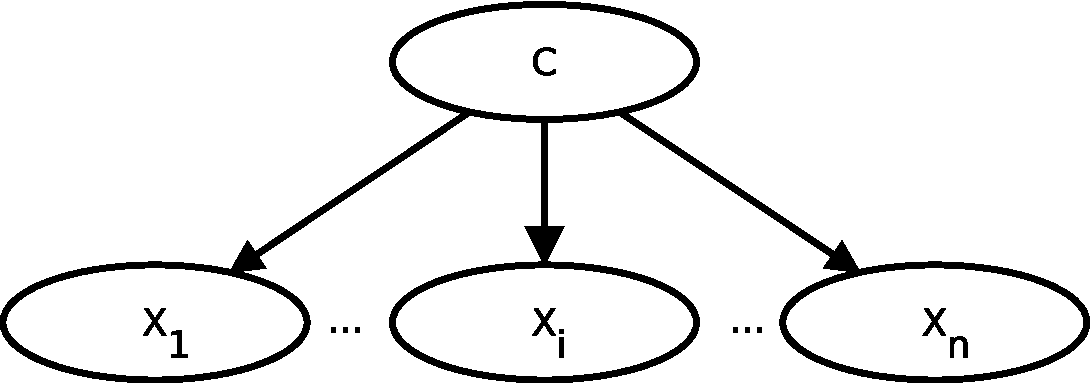
\includegraphics[scale=0.4]{fig/bn-naive-bayes}
        \caption{General Naïve Bayes model in which holds $\forall i \neq j: X_i \perp X_j \mid C$}
        \label{fig:bn_d-separation_a}
    \end{subfigure}
    \qquad\qquad\qquad
    \begin{subfigure}[b]{0.42\linewidth}
        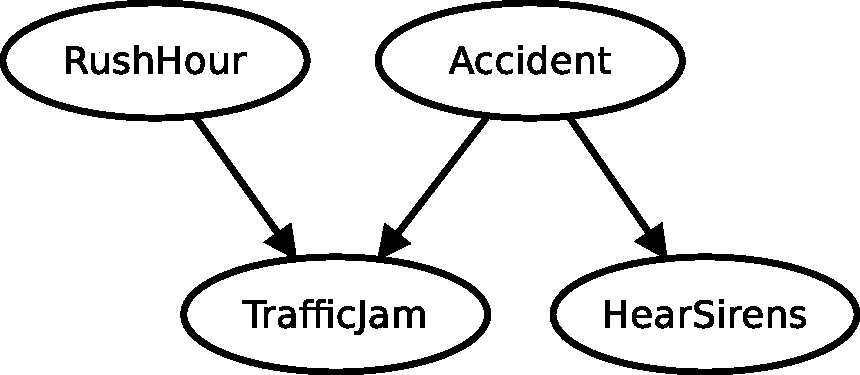
\includegraphics[scale=0.4]{fig/bn-d_sep-traffic}
        \caption{Example of an activated V-structure, $R\not\perp H \mid T$ (active trail $R-T-A-H$)}
        \label{fig:bn_d-separation_traffic}
    \end{subfigure}
  
    \begin{subfigure}[b]{0.42\linewidth}
        \vspace{0.5cm}
        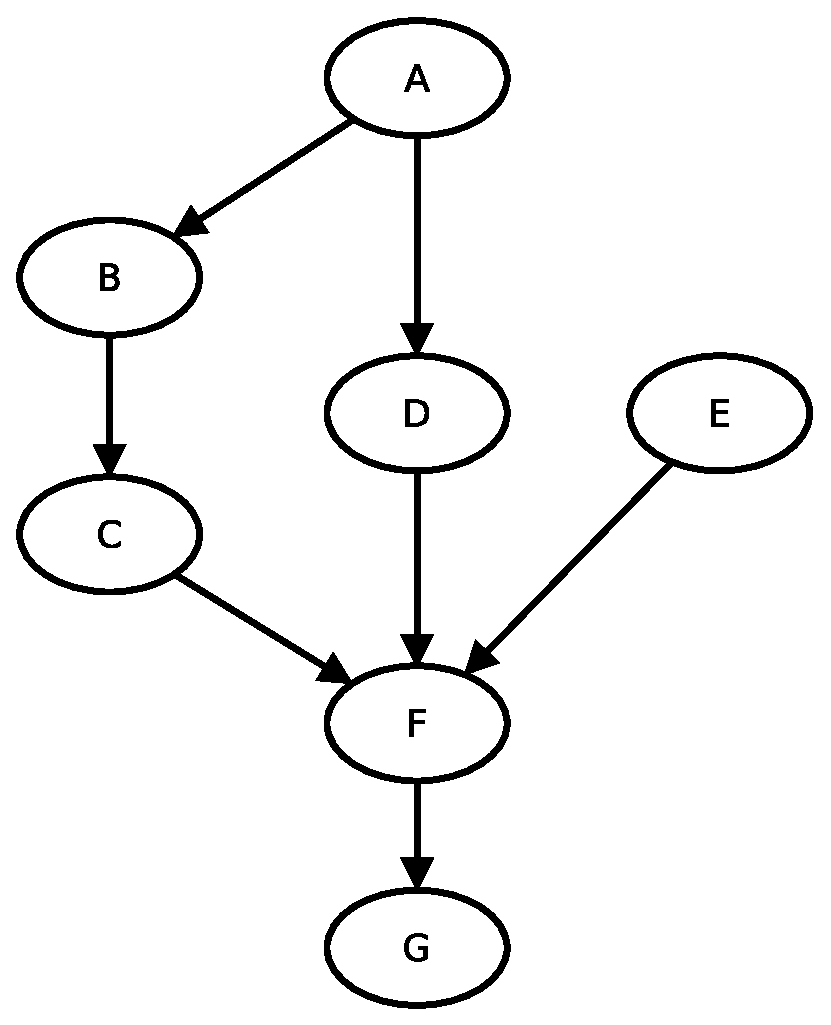
\includegraphics[scale=0.4]{fig/bn-d_sep-abstract}
        \caption{A more complicated network with multiple possible trails and other interesting cases.}
        \label{fig:bn_d-separation_abstract}
    \end{subfigure}
    
    \caption{Networks for demonstration of d-separation and flow of influence.}
    \label{fig:bn_d-separation}
\end{figure}
\end{center}

It might be useful to explicitly point out what the notation $P(X_i \mid Parents(X_i))$ tells us in context of d-separation. It is a fact frequently used in mathematical derivations in context of BNs that, when given all parents $Parents(X_i)$ of a variable $X_i$, the variable is independent of all its indirect parents in the network. In Markov chain Monte-Carlo sampling we will also introduce so called \term{Markov blanket} of variable $X$ which is minimal set of variables such that $X$ is conditionally independent on any other variable in the network given its Markov blanket.













\section{Inference in Bayesian networks}
There are several types of queries that might be asked in context of a Bayesian network. Most frequently, by inference in BNs is meant computing the posterior probability distribution for a set of query variables $\vars{X}$ given values $\vars{e}$ of evidence variables $\vars{E}$. Mathematically, the task is to compute the probability distribution $P(\vars{X} \mid \vars{e})$. Another type of query is so called \term{maximum a~posteriori} (abbreviated as MAP) that is finding $arg\ max_\vars{X} P(\vars{X} \mid \vars{e})$. MAP is basically used for finding out the most probable cause (concrete assignment of variables $\vars{X}$) for observation $\vars{e}$. A practical example could be getting the most probable word (sequence of letters) that corresponds to classifier output for a segmented picture containing that word. Although this is an example more frequently used in context of Markov networks.

Inference in a BN may be carried out in many ways depending on nature of the query and precision requirements. Exact inference is relatively straightforward in terms of mathematical description and naive algorithmic implementation but exhibits serious running-time disadvantage\,--\,exponential running time in the number of variables in the worst case. On the other hand, approximate inference methods allow us to answer queries more quickly but precision of the solution may be questionable, especially for very rare events.

\todo{maybe show types of queries\,--\,diagnostic, causal, intercausal, mixed?~\cite[p.~448]{russell_norvig_ed2}}

\subsection{Sum-product}
Probably the simplest method for computing a conditional probability query is called sum-product. The problem at hand is to compute conditional probability distribution $P(\vars{X} \mid \vars{e})$ where $\vars{X}$ is one or more variables, $\vars{e}$ is an assignment to evidence variables $\vars{E}$ and $\vars{Y}$ variables that are neither query nor evidence variables. The query is computed according to Bayes' theorem as follows:
\begin{equation*}
P(\vars{X} \mid \vars{e})
 = \frac{P(\vars{X}, \vars{e})} {P(\vars{e})}
 = \frac{\sum_\vars{Y} P(\vars{X}, \vars{y}, \vars{e})}{\sum_{\vars{X},\vars{Y}} P(\vars{x}, \vars{y}, \vars{e})}
\end{equation*}
The denominator is constant and since $P(\vars{X} \mid \vars{e})$ has to be a probability distribution, we can simply omit the denominator and in the end normalize numerator by some constant $\alpha$. Hence we can write
\begin{equation*}
P(\vars{X} \mid \vars{e})
 = \alpha \sum_\vars{Y} P(\vars{X}, \vars{y}, \vars{e})
\end{equation*}
Computation of this expression using the sum-product method means performing four steps:
\begin{enumerate}
	\item reducing all factors in the Bayesian network by evidence $\vars{e}$,
	\item multiplying reduced factors all together producing single joint factor $P(\vars{X},\vars{Y},\vars{e})$ which is not a probability distribution because, in general, all values of the factor don't sum to one,
	\item marginalizing over the variables $\vars{Y}$ (non-query and non-evidence variables) and finally
	\item renormalizing the resulting factor, obtaining the joint probability distribution $P(\vars{X},\vars{e})$.
\end{enumerate}

Every item of the sum in numerator, ie. probability of every possible assignment to variables $\vars{Y}$, can be written according to the joint probability distribution represented by a~BN (definition~\eqref{eq:bn_joint}) as a~product of conditional probabilities of all variables in given BN. This explains the name of this inference method\,--\,we effectively compute many products of conditional probabilities and sum over variables $\vars{Y}$.

Sum-product inference algorithm has, by its nature, exponential running time in the number of variables because it effectively generates the whole joint probability distribution encoded by a given Bayesian network and the size of a table representing any joint probability distribution has been earlier shown to be exponential in the number of variables. Because of this quality, the sum-product method is suitable only for inference in considerably small networks.

\begin{comment}
\uncertain{
Formally, exact number of operations carried out in the nominator sum during the sum-product inference can be determined as follows. Let $m$ be the number of all variables, let $n$~be the number of non-query and non-evidence variables $\vars{Y}$ and let $k$~be the number of possible assignments to a variable. The numerator summation unrolls to $k^n$ items, each item being a product of all $m$ factors which means $k^n (m-1)$ multiplications and $k^n - 1$ additions. Therefore the overall running time is roughly $O(m k^n)$.}
\end{comment}


\subsection{Variable elimination}
Variable elimination algorithm can be seen as a somewhat smarter implementation of the sum-product algorithm explained above. Again, we answer the given query by multiplying all factors of the BN and summing out $\vars{Y}$ variables. The innovative ideas behind variable elimination are:
\begin{itemize}
	\item Suppose we sum over many variables in a product of factors, say one of these variables is $V$. Then factors whose scopes don't contain $V$ are irrelevant for the summation over~$V$ and hence these factors can be factored out in front of the summation over~$V$. This way we can push all summations as far to the right as possible, so that each summation is done only over product of factors containing the variable $V$ being summed out. What is the benefit for us? It can be shown~\cite{pgm} that running time of variable elimination depends on the size of the largest immediate factor during the summing-out process. When we sum only over product of factors containing variable $V$, the resulting immediate factor is the smallest possible. Because problem of determining the optimal order of elimination is NP-hard, greedy heuristics are usually used instead~\cite{pgm}.
	\item By definition of a conditional probability distribution, it holds for any instantiation of parent variables that $\sum_V P(v \mid Parents(V)) = 1$. So, when computing posterior probability distribution $P(\vars{X} \mid \vars{e})$, any node (factor) $V$ that is not an ancestor of a~query or evidence variable can be omitted because, thanks to the order of elimination of variables, the term $\sum_V P(v \mid Parents(V))$ will be the rightmost summation (the innermost). So summing out $V$ is equivalent to totally excluding variable $V$ from the BN. Implementation can be recursively done in the way of eliminating all leaf nodes that are not in $\vars{X} \cup \vars{E}$ and performing the same operation for as long as some node gets removed~\cite[p.~510]{russell_norvig_ed2}.
\end{itemize}

%\todo{řeči kolem, algoritmus, časová složitost, kliky}

Running time of the variable elimination algorithm in polytrees is $O(n)$~\cite[p.~510]{russell_norvig_ed2}, therefore it is a good method for answering individual queries $P(X \mid \vars{e})$ where $X$ is a single variable. Analogically, we can effectively compute probability distribution for small number of query variables $\vars{X}$ by computing individual distributions $P(X_i \mid \vars{e})$ for all $X_i \in \vars{X}$ and returning $P(\vars{X} \mid \vars{e}) = \prod_i P(X_i \mid \vars{e})$.

Running time in multiply connected networks is exponential in general but it can be coped with by clustering algorithms that transform multiply connected network into a~polytree which can be processed in linear time.

\subsection{Belief propagation}
Belief propagation~\cite{pgm} is an approximate inference algorithm from the family of so called \term{message passing algorithms}. The main idea is that nodes in the BN exchange information about their believes (probability distributions affected by evidence) and the whole network converges to some solution close to true posterior probability. As methods from this family are far from trivial and they are not the aim of this thesis, we will not pay deeper attention to them.
\begin{comment}
\note{Cluster graphs and \term{running intersection property}: Nodes $C_i \subseteq \lbrace X_1, \dots, X_n \rbrace$ and sepsets $S_{i,j} \subseteq C_i \cup C_j$ such that for each factor $\phi$ exists $C_i$: $scope(\phi) \subseteq C_i$.
For each variable $X$ the nodes $C_i$ and sepsets containing $X$ form a tree (ie. no cycle and single unbroken component)\,--\,cycle would mean that a node would get information about variable $X$ twice and the probabilities would go up and up. If some node with $X$ would be isolated from others, it would not get the belief updates. Bethe cluster automatically satisfies the running intersection property.}
\end{comment}


\subsection{Sampling methods}
Monte Carlo methods (or particle methods) are stochastic methods of inference based on sampling the probability distribution induced by a BN. There are three main sampling methods: \term{direct sampling}, \term{rejection sampling} and \term{likelihood weighting}. All these methods basically generate a sufficient number of independent samples and then compute simple statistics over these samples. In general, relative precision of Monte Carlo methods is proportional to $1/\sqrt{N}$, where $N$ is the number of samples.

\subsubsection{Direct sampling}
Direct sampling is a method for computing probability distribution in the form $P(\vars{U} \mid \vars{V})$, ie. without any known evidence. Of course must hold that $\vars{U} \neq \emptyset \wedge \vars{U} \cap \vars{V} = \emptyset$. For the sake of clarity of formulas we will consider $\vars{X} = \vars{U} \cup \vars{V}$ and compute the probability distribution $P(\vars{X})$ from which the conditional distribution $P(\vars{U} \mid \vars{V})$ can be easily obtained using Bayes' rule. This simplification is applied to all sampling methods further described. 

Direct sampling produces a number of samples, ie. of concrete events according to the probability distribution induced by the given BN and then for every assignment $\vars{x}$ computes its probability as $P(\vars{x}) = N_\vars{x} / N$, where $N_\vars{x}$ is the number of samples in which variables $\vars{X}$ have the values $\vars{x}$ and $N$ is the number of all samples generated.

A single sample is generated as follows. First randomly assign values to variables with no parents according to their probability distributions. Then choose a variable $V$ such that all of its parents have already been instantiated and randomly assign a value to $V$ according to the probability distribution $P(V \mid parents(V))$ where $parents(V)$ are the concrete values of its parents in current sample. Repeat this step until all variables have been instantiated, thereby obtaining a~sample. The process can easily be done if we first compute topological sort of the BN and then sample variables in ascending order.

It can be shown~\cite[p.~491]{pgm} that to obtain an estimate with error bounded by $\epsilon$ with probability at least $1-\delta$ we need to generate $M$ samples:
\begin{equation*}%\label{eq:sampling_accuracy}
M \geq \frac{\ln(2 / \delta)}{2 \epsilon ^ 2}
\end{equation*}
Problem is that for a very unlikely event we may not generate a single sample and therefore the obtained probability distribution would indicate that this event is impossible (its probability equals to zero). Still it would be a sound result within the error estimate $(\epsilon, \delta)$.

\subsubsection{Rejection sampling}
Direct sampling presented earlier doesn't allow for any evidence. Rejection sampling could be viewed as a simple extension of direct sampling for computing posterior probability distribution with evidence $\vars{E} = \vars{e}$, ie. distribution in the form $P(\vars{X} \mid \vars{e})$. The idea is to exclude samples inconsistent with evidence $\vars{e}$ meaning that when an evidence variable is instantiated during the production of a sample, the sample is discarded unless the randomly assigned value corresponds with the observed value. The desired distribution is determined by computing $P(\vars{x} \mid \vars{e}) = N_{\vars{x}, \vars{e}} / N_\vars{e}$ for every instantiation of $\vars{X}$.

This simple approach bears the disadvantage that if the observed evidence is very unlikely then many samples get discarded and hence a lot of computational time is wasted because rejected samples don't contribute to the final probability distribution estimate. Unfortunately, when considering somewhat uniform distribution, the probability $P(\vars{e})$ decreases exponentially with the number of observed variables (eg. with symptoms of a~patient) and by the same rationale the number of samples that are not rejected decreases just as rapidly.

\subsubsection{Likelihood weighting (\todo{implementation note: compute $P(\vars{X}\cup\vars{Y}\mid\vars{e})$ and renorm.})}
Rejection sampling described earlier can theoretically be used for answering queries of the form $P(\vars{X} \mid \vars{e})$ but the number of rejected samples may be unbearable in practice. Likelihood weighting method copes with this problem by forcing every sample to be consistent with observed evidence, ie. by artificially setting variables $\vars{E}$ to $\vars{e}$. Then, of course, not every sample is equally likely, so we cannot determine $P(\vars{x} \mid \vars{e})$ by simply dividing number of samples $N_{\vars{x},\vars{e}}$ by $N_\vars{e}$. For each sample we need some additional information which is the probability of assigning values $\vars{e}$ to evidence variables given values of other variables in the current sample~\cite[p.~514]{russell_norvig_ed2}. Let $\vars{Y}$ denote set of all variables in a BN other than the variables $\vars{X} \cup \vars{E}$. Then we can state that weight of a sample $\vars{x},\vars{e}, \vars{y}$ is $w_{\vars{x},\vars{e}, \vars{y}} = \prod_\vars{E} P(e \mid parents(E))$ where $parents(E_i)$ denotes assignment to variables $Parents(E_i)$ according to the given sample $\vars{x},\vars{e}, \vars{y}$.

The sampling algorithm needs to be changed in the following way. First of all, the counters of samples won't be integral but real. Also, when generating a~new sample we will keep not only the values of variables but also weight of the sample. When generating a new sample, first we set the weight of the current sample to 1. Then we sample all variables in topological order. For a non-evidence variable $X_i$ we proceed as in the case of direct sampling\,--\,randomly assign a value $x_i$ according to the probability distribution $P(X_i \mid parents(X_i))$ which is governed by the current instantiation of $X_i$'s parents. When we encounter an evidence variable $E_i$, we set it to value $e_i$ according to the given evidence $\vars{e}$ and multiply weight of the current sample by $P(e_i \mid parents(E_i))$. When a sample is completed we increase the counter $C_{\vars{x},\vars{e}}$ by the weight of the generated sample. The final probability distribution is computed as follows:

\begin{comment}
\begin{equation}\label{eq:weighted_sampling}
    P(\vars{x} \mid \vars{e})
    = \frac
        {w_{\vars{x},\vars{e}} \cdot N_{\vars{x},\vars{e}}}
        {\sum_\vars{X} (w_{\vars{x},\vars{e}} \cdot N_{\vars{x},\vars{e}})}
\end{equation}
\end{comment}

\begin{equation}\label{eq:weighted_sampling}
    P(\vars{x} \mid \vars{e})
    = \frac{C_{\vars{x},\vars{e}}}{C_{\vars{e}}}
\end{equation}

Because weighted sampling might not be as obvious as direct and rejection sampling, I will try to elaborate and provide some insight. The key difference to previous sampling methods is that we want each sample to contribute to the final probability distribution estimate but then each generated sample cannot be accounted for by the same amount. Therefore the weight of a sample is used which literally bears the information how likely is the observed evidence $\vars{e}$ in that sample (for direct and rejection sampling the weight would be always one).
To understand weighted sampling better I have devised  a formal derivation of the formula~\eqref{eq:weighted_sampling}. Let $\vars{Y}$ denote set of all variables in a BN other than the variables $\vars{X} \cup \vars{E}$. First we will derive an alternative expression for $P(\vars{x}, \vars{e})$ which will be useful later.

\begin{eqnarray}
    P(\vars{x}, \vars{e})
    & = & \sum_\vars{Y} P(\vars{x}, \vars{e}, \vars{y}) \nonumber\\
    & = &
       \sum_\vars{Y} \Bigl( \prod_{E_i \in \vars{E}} P(e_i \mid parents(E_i)) \prod_{X_i \in \vars{X}} P(x_i \mid parents(X_i)) \prod_{Y_i \in \vars{Y}} P(y_i \mid parents(Y_i)) \Bigr) \nonumber\\
    & \approx &
       \sum_\vars{Y} \Bigl( w_{\vars{x},\vars{e},\vars{y}} \cdot \frac{N_{\vars{x},\vars{e},\vars{y}}}{N_{\vars{e},\vars{y}}} \cdot \prod_{Y_i \in \vars{Y}} P(y_i \mid parents(Y_i)) \Bigr) \nonumber\\
    & \approx &
       \sum_\vars{Y} \Bigl( w_{\vars{x},\vars{e},\vars{y}} \cdot \frac{N_{\vars{x},\vars{e},\vars{y}}}{N_{\vars{e}} \cdot \prod_{Y_i \in \vars{Y}} P(y_i \mid parents(Y_i))} \cdot \prod_{Y_i \in \vars{Y}} P(y_i \mid parents(Y_i)) \Bigr) \nonumber\\
    & = &
        \sum_\vars{Y} \Bigl( w_{\vars{x},\vars{e},\vars{y}} \cdot \frac{N_{\vars{x},\vars{e},\vars{y}}}{N_{\vars{e}}} \Bigr)
        = \frac{1}{N_\vars{e}} \cdot \sum_\vars{Y} \Bigl( w_{\vars{x},\vars{e},\vars{y}} \cdot N_{\vars{x},\vars{e},\vars{y}}\Bigr) \label{eq:weighted_sampling_P_x_e}
\end{eqnarray}

Lets go through the derivation step by step. The first line merely states we have to marginalize over all the remaining variables $\vars{Y}$ in the network.
On the second line we just rewrote the joint probability according to the definition of a~Bayesian network.
On the third line we replaced exact probabilities by their sampled equivalents (therefore the approximation symbol instead of equality). Namely weight of the sample $w_{\vars{x},\vars{e},\vars{y}}$ is equal to the probability $P(\vars{e} \mid \vars{x},\vars{y})$ and ratio $N_{\vars{x},\vars{e},\vars{y}} / N_{\vars{e},\vars{y}}$ approximately equals to $P(\vars{x} \mid \vars{e},\vars{y})$.
On the forth line we needed to express the number $N_{\vars{e},\vars{y}}$ of samples with concrete values $\vars{e},\vars{y}$ using the probability $P(\vars{y} \mid \vars{x},\vars{e})$ and the total number of samples generated $N_\vars{e}$ (remember that in weighted sampling all samples are consistent with the evidence, so $N_\vars{e}$ really is the total number of samples).
Finally, on the fifth line the big products over $\vars{Y}$ cancel out and we obtain the final expression for $P(\vars{x},\vars{e})$.
Now lets make some use of it:

\begin{eqnarray*}
    P(\vars{x} \mid \vars{e})
    & = &
      \frac
        {P(\vars{x},\vars{e})}
        {P(\vars{e})} = \frac{P(\vars{x},\vars{e})}{\sum_\vars{X} P(\vars{x},\vars{e})}
    = \frac
        {\frac{1}{N_\vars{e}} \cdot \sum_\vars{Y} \Bigl( w_{\vars{x},\vars{e},\vars{y}} \cdot N_{\vars{x},\vars{e},\vars{y}}\Bigr)}
        {\sum_\vars{X} \frac{1}{N_\vars{e}} \cdot \sum_\vars{Y} \Bigl( w_{\vars{x},\vars{e},\vars{y}} \cdot N_{\vars{x},\vars{e},\vars{y}}\Bigr)} \\
    & = &
      \frac
        {\sum_\vars{Y} \Bigl( w_{\vars{x},\vars{e},\vars{y}} \cdot N_{\vars{x},\vars{e},\vars{y}}\Bigr)}
        {\sum_\vars{X} \sum_\vars{Y} \Bigl( w_{\vars{x},\vars{e},\vars{y}} \cdot N_{\vars{x},\vars{e},\vars{y}}\Bigr)} \\
    & = & \frac{C_{\vars{x},\vars{e}}}{\sum_\vars{X} C_{\vars{x},\vars{e}}}
      = \frac{C_{\vars{x},\vars{e}}}{C_{\vars{e}}}
\end{eqnarray*}

On the first line we rewrote the conditional probability using Bayes' rule and then we substituted for $P(\vars{x},\vars{e})$ the expression~\eqref{eq:weighted_sampling_P_x_e} derived earlier.
On the second line the $1/N_\vars{e}$ cancel out.
To understand the third line we need to revisit how the weighted sampling works, especially what values are accumulated in a counter $C_{\vars{x},\vars{e}}$ and how. There are two key points. First, the weight $w_{\vars{x},\vars{e},\vars{y}}$ of each sample $\vars{x},\vars{e},\vars{y}$ is added to the counter $C_{\vars{x},\vars{e}}$ exactly $N_{\vars{x},\vars{e},\vars{y}}$-times. The second critical observation is that the counters don't care for values of the $\vars{Y}$ variables, so weights of two samples $\vars{x},\vars{e},\vars{y'}$ and $\vars{x},\vars{e},\vars{y''}$ are by the weighted sampling algorithm added to the same counter $C_{\vars{x},\vars{e}}$; this is effectively the same as marginalizing over the variables $\vars{Y}$ (ie. summing $\vars{Y}$ out) during the sampling.
  Combining these two pieces of information we conclude that the second and the third line have to equal. Formal derivation of the formula~\eqref{eq:weighted_sampling} for weighted sampling is now complete.

\medskip

I believe that the sampling process can furthermore be accelerated by omitting a set of variables, denoted $\vars{Z}$, from the network being sampled where $\vars{Z}$ is maximal set of variables satisfying the following two conditions: (1) $\vars{Z} \cap (\vars{X} \cup \vars{E}) = \emptyset$, (2) no direct or indirect child of any variable from $\vars{Z}$ is in $\vars{X} \cup \vars{E}$. Rationale behind this is the same as in the variable elimination algorithm\,--\,when computing the final probability distribution, we effectively sum out variables $\vars{Z}$ and it is irrelevant what random values they are assigned because if two samples differ only in the values of $\vars{Z}$ then these samples contribute to the same counter $C_{\vars{x},\vars{e}}$ and also $\vars{Z}$ don't affect weights of the samples as $\vars{Z} \cap \vars{E} = \emptyset$. This observation is applicable to direct and rejection sampling as well.

Important drawback of likelihood weighting is that it doesn't account well for evidence in leaf nodes or near to them. This is because in that case we effectively sample the prior probability distribution and finally we modify weight of the generated sample by evidence but the sampling process is most of the time unaffected by the evidence and virtually only weights of samples take evidence into account. So, for a very rare instantiation of evidence variables (eg. for some rare and/or big set of symptoms) all of the generated samples might have very small weight and, in case of medical diagnosis, no sample representing the "real cause" of observed evidence might be generated at all. Once again, this is because we sample prior probability distribution rather than posterior and these two distributions may be very different~\cite[p.~503]{pgm}.

\subsection{Markov Chain Monte Carlo}
The likelihood weighting method presented earlier doesn't account well for evidence near leaf nodes, ie. for so called \term{evidential reasoning}. Markov Chain Monte Carlo (MCMC) is also a stochastic method that generates samples but rather than generating each sample completely from scratch it modifies the last sample by resampling one of the non-evidence variables. This way, the information about all evidence variables propagates through the network and with time we get closer to the true posterior probability distribution.

To explain how the MCMC algorithm works we first need to introduce so called \term{Markov blanket} of a~variable $X$ (see Figure~\ref{fig:bn-markov-blanket}), denoted $MB(X)$. The Markov blanket of $X$ is the minimal set of variables other than $X$ such that $X$ is conditionally independent of all other variables in the BN given $MB(X)$. It is fairly obvious that the Markov blanket includes variables $Parents(X)$ and direct children of $X$, denoted $Children(X)$, because there is a direct connection between these variables and $X$. Furthermore, $MB(X)$ also needs to include parents of every variable in $Children(X)$ because observing any of the children $C_i$ activates a V-structure and $X$ becomes conditionally dependent on $Parents(C_i)$ given $C_i$. Formally the Markov blanket could be defined as follows:
\begin{equation*}
MB(X) = Parents(X) \cup Children(X) \cup \!\!\!\!\!\!\!\! \bigcup_{C \in Children(X)} \!\!\!\!\!\!\!\!\!\!\!\! Parents(C)
\end{equation*}

\begin{center}
\begin{figure}[h]
    \begin{center}
    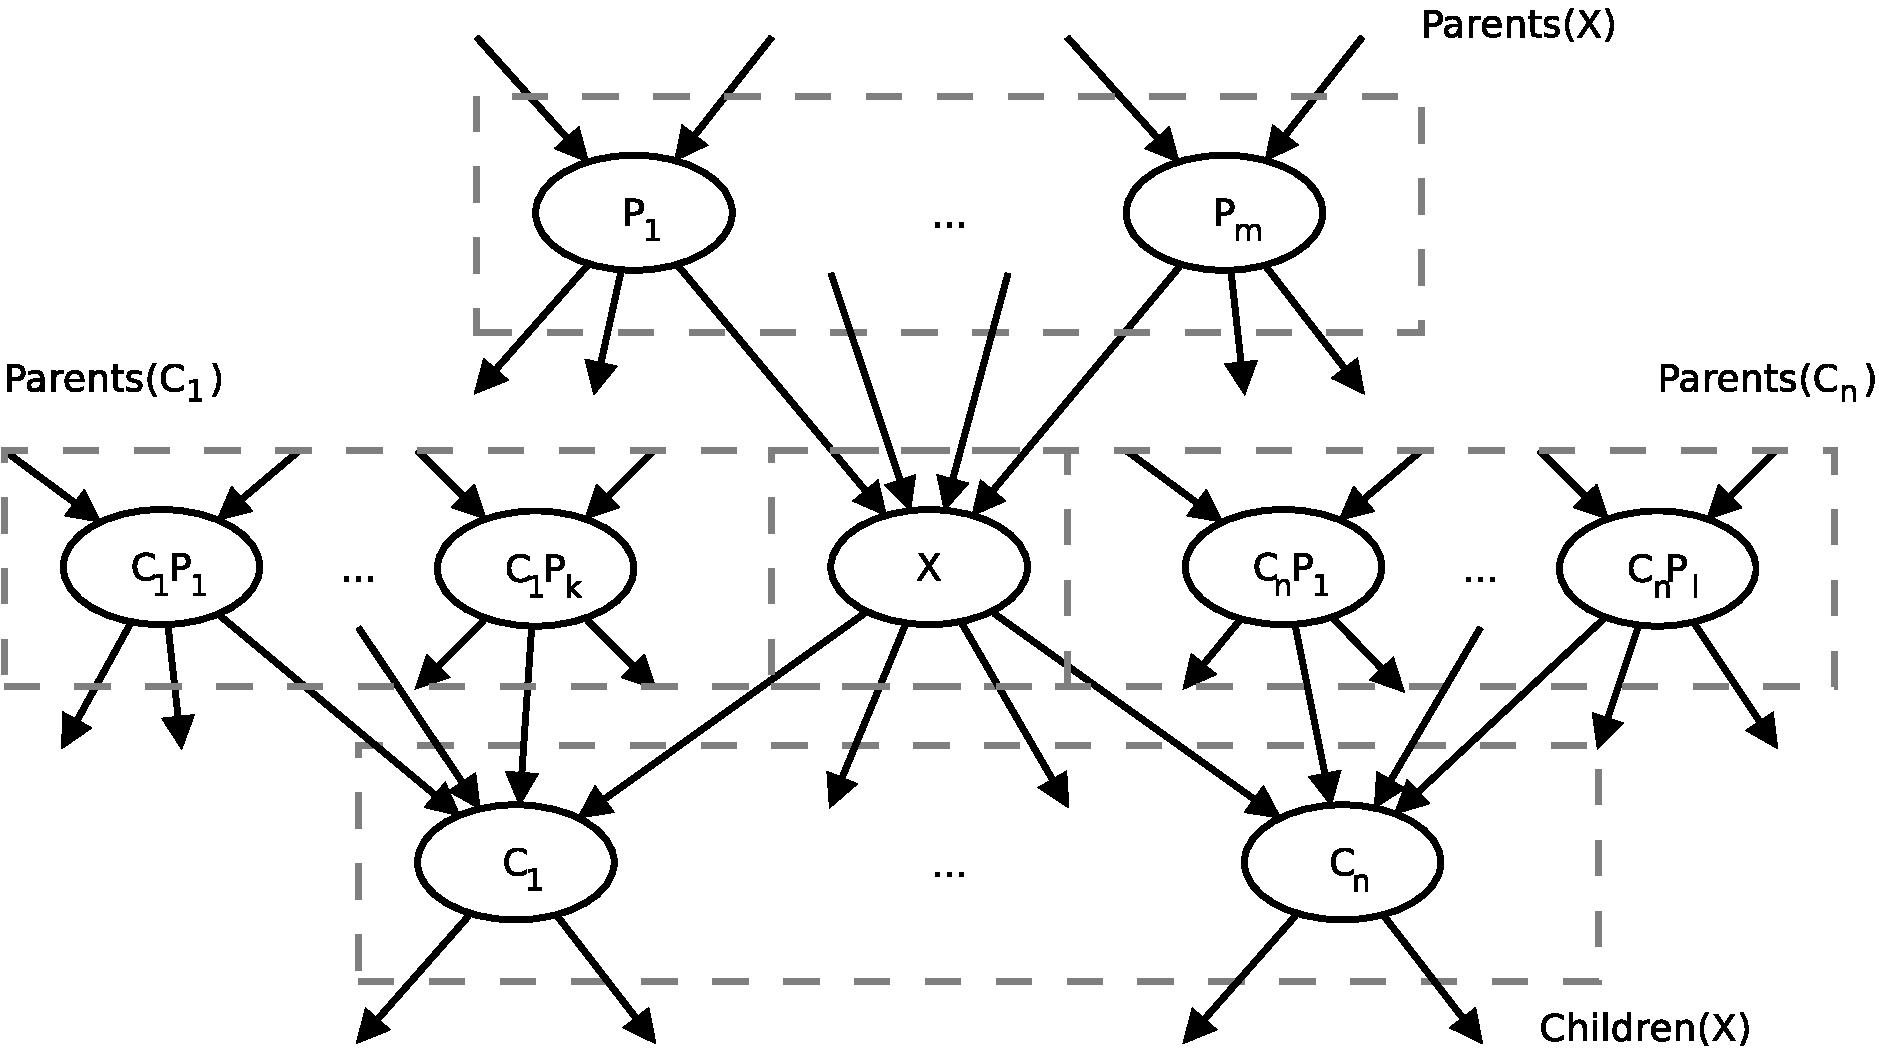
\includegraphics[scale=0.4]{fig/bn-markov_blanket}
    \end{center}
    \caption{Markov blanket $MB(X)$ of variable $X$ consists of all variables in this figure except $X$.}
    \label{fig:bn-markov-blanket}
\end{figure}
\end{center}

Now, in order to resample some variable $X$ and thereby to produce a new MCMC sample, we need to compute the probability distribution $P(X \mid mb(X))$ and sample new value of $X$ from this distribution. In a sense, Markov blanket of variable $X$ defines context of the resampling, ie. all the variables whose values we need to know.

The MCMC algorithm~\cite[p.~516]{russell_norvig_ed2} starts by producing one sample consistent with the evidence, eg. by one iteration of likelihood weighting with the weight discarded. Then we repeat the following: For each non-evidence variable $V$ we resample this variable from the current distribution $P(V \mid mb(V))$ producing a new sample with value of variable $V$ potentially changed. For the new sample we increase the corresponding counter $N_{\vars{x},\vars{e}}$ and proceed with resampling of another variable. The distribution $P(V \mid mb(V))$ needed for resampling of variable $V$ can be obtained by computing $P(v \mid mb(V))$ for every $v$ as follows:
\begin{equation*}
    P(v \mid mb(V)) = \alpha \cdot P(v \mid parents(V)) \!\!\!\!\!\!\!\! \prod_{C_i \in Children(V)} \!\!\!\!\!\!\!\!\!\!\!\! P(c_i \mid parents(C_i))
\end{equation*}
where $\alpha$ is a normalizing constant. Note that $mb(\cdot)$ and $parents(\cdot)$ denote concrete instantiation of respective variables in the current sample.

Intuition behind the MCMC algorithm is that the sampling process will reach a dynamic equilibrium in which time spent with each instantiation of non-evidence variables (ie. the counter of samples $N_{\vars{x},\vars{e}}$) is proportional to the probability of this instantiation. More formally, MCMC is based on state space induced by a BN represented by a Markov model~\cite[p.~516]{russell_norvig_ed2} but this theory is not necessary for understanding the MCMC inference method.

%\note{pgm 541+ has good notes of other papers} % SP

\begin{comment}
$\pi(x)$ is the stationary distribution (ustálený)

works for regular Markov chains ($\exists k \forall x, x':$ z $x$ do $x'$ se lze dostatat přesně v $k$ krocích s nenulovou pstí)
\end{comment}












\section{Model learning}
So far, we have been reasoning about Bayesian networks that were already given to us, so that both the structure of the BN and the CPDs associated with nodes were known. Now we are going to examine the problem of creating a Bayesian network so that the probability distribution it induces somehow corresponds to the real probability distribution of the target domain.

Basically, there are two approaches to creating a BN. First option is to cooperate with an expert of target domain who can make correct dependency and independency assumptions and provide us with conditional probability distributions, ie. with CPDs to all nodes. The other approach is to use automated techniques for creating models based on a big dataset. The dataset can be viewed as a set of samples of the target probability distribution $P*$ which we attempt to reconstruct. The aim is to create a model $\tilde{\mathcal{M}}$ such that the probability distribution $P_{\tilde{\mathcal{M}}}$ induced by $\tilde{\mathcal{M}}$ is "very close" to the original distribution $P*$.

Complete construction of a BN through cooperation with an expert is problematic because, for a non-trivial BN, the task often requires significant time (several months~\cite{pgm}), the expert might not correctly capture CPDs, especially for nodes with large number of parents and furthermore there might not even be an expert of the target domain at all. On the other hand, automated techniques of model construction are constrained by limited computational power and, more importantly, by the size of the supplied dataset. As will be shown later, we encounter classical problem of overfitting and bias-variance trade-off present in the whole artificial intelligence and machine learning. In practice we often combine these two approaches in the way that an expert defines structure (all variables and their dependencies) and an automated process determines CPDs by supplied dataset.

%\todo{maybe include general metrics?} % SP

\section{Parameter estimation}
Goal of parameter estimation is to supply CPDs to a BN whose structure is already known. In order for the estimation to be reasonably correct, we need to have sufficiently large dataset wrt. complexity of the BN structure.


\subsection{Maximum likelihood estimation}
Maximum likelihood estimation views the dataset $\mathcal{D}$ as a set of independent samples $x_1, \dots, x_m$ obtained from a~parametrized probability distribution with parameter $\Theta$. The parameter $\Theta$ can be viewed as a vector of entries of all CPDs if the probability distribution was represented by a BN. Core of the maximum likelihood estimation is to choose $\Theta$ in such a way that the probability of obtaining samples $x_1, \dots, x_m$ from the parametrized distribution is maximal. Formally $\Theta = \arg \max P(\mathcal{D} \mid \Theta)$ where $P(\mathcal{D} \mid \Theta)$ is called \term{likelihood function}.

Let's inspect a simple example of $m$ coin tosses $x_1, \dots, x_m$ with a biased coin for which $P(X = heads) = \theta$ (inspired by~\cite{pgm}). Let's suppose we get $H$ times heads and $T$ times tails. Then we can write $P(x_1,\dots,x_m \mid \theta) = \theta^H (1 - \theta)^T$ because the coin tosses are mutually independent given $\theta$. The task of maximizing the expression $\theta^H (1 - \theta)^T$ is equivalent to maximizing its logarithm $H \cdot \ln(\theta) + T \cdot \ln(1 - \theta)$. The equation $\frac{\partial}{\partial\theta} \ H \cdot \ln(\theta) + T \cdot \ln(1 - \theta) = 0$ yields global maximum $\theta = H / (H + T)$ which is a fairly intuitive conclusion\,--\,probability of heads is the number of times we got heads divided by the number of all tosses. Similar formula can be obtained for a~general multinomial variable.

Now suppose we want to compute probability distribution $P(X \mid Parents(X))$ for some node $X$ according to our dataset, ie. to compute the CPD of that node.
Maximum likelihood estimation is, as demonstrated earlier, an intuitive approach when we partition the dataset to disjoint subsets, each for a concrete instantiation of variables $\lbrace X \rbrace \cup Parents(X)$. Then CPD entry $P(X=x_i \mid Parents(X) = \vars{p_j})$ is computed as the ratio $N_{x_i,\vars{p_j}} / N_{\vars{p_j}}$. Potential problem with this approach is that the number of subsets grows exponentially with the number of parents and hence the estimated CPD looses precision. This exponential explosion of possible instantiations is called \term{fragmentation} and it is one of the main problems of learning BNs from data. Because of fragmentation, a perfect model capturing all dependencies between variables might be outperformed by a simpler and wrong model just because we don't have sufficient amount of data to accurately compute CPDs for the more complicated structure\footnote{Such observation has often been made, for example, with the Naïve Bayes model which assumes that any two effect variables are independent given the cause variables. Such assumption is seldom justified, nevertheless Naïve Bayes models have proved themselves to perform well.}~\cite{pgm}. This is a~typical AI problem of overfitting. In extreme cases $N_{x_i,\vars{p_i}}$ could be zero which is in most cases very wrong. This can be prevented by applying the Laplace's correction commonly used in context of Naïve Bayes classifier.


\subsection{Bayesian estimation}
An important drawback of the maximum likelihood estimation presented earlier is that it doesn't really account for the size of the dataset\,--\,small dataset may not have enough samples for every instantiation of every variable and its parents and the dataset might also be noisy. The key idea of Bayesian estimation is to view the parameters themselves (ie. CPDs) as random variables with some prior distribution and then, according to the supplied dataset, compute the posterior distribution over parameters which will be our estimated CPDs. So, parameter learning is in this case a type of inference.
More formally, we define a~prior distribution $P(\Theta)$ over parameters $\Theta$ with some degree of strength of this initial distribution (will be explained later) and then, using the Bayes' rule, compute the posterior probability distribution $P(\Theta \mid \mathcal{D}) \propto P(\mathcal{D},\Theta) P(\Theta)$ as we get more empirical data. This way the Bayesian estimation can, for example, distinguish between rolling a~six three times out of eight throws, which may be accounted just to statistical noise, and rolling a six 3\,000 times out of 8\,000 throws. It is clear that these two datasets tell us something different about the die, although probability of rolling a six, according to the maximum likelihood estimation, is $3/8$ in both cases.

The exact mathematical derivation~\cite[p.~733]{pgm} of Bayesian parameter estimation formulas is based on \term{Dirichlet distribution}$(\alpha_1,\dots,\alpha_k)$. The derivation is not trivial and also is not needed further in this thesis, so we jump straight to the practical conclusions and interpretations. For a~given dataset $\mathcal{D}$ and hyperparameters $(\alpha_1, \dots, \alpha_k)$ the probability of variable $X$ having value $x_i$ is given as follows (for a node without and with parents):

\begin{equation*}
    \begin{array}{rcl}
    P(X = x_i \mid \mathcal{D}) &
     = &
     \displaystyle\frac
        {\alpha_{x_i} + N_{x_i}}
        {\sum_j (\alpha_{x_j} + N_{x_j})}\\
        & & \\
    P(X = x_i \mid Parents(X) = \vars{p_i}, \mathcal{D}) &
     = &
     \displaystyle\frac
        {\alpha_{x_i \mid \vars{p_i}} + N_{x_i, \vars{p_i}}}
        {\sum_j (\alpha_{x_j \mid \vars{p_i}} + N_{x_j, \vars{p_i}})}
    \end{array}
\end{equation*}
where the hyperparameter $\alpha_{x_i}$ can be viewed as count of imaginary samples $x_i$ (also called \term{pseudo-samples}), similarly for $\alpha_{x_i \mid \vars{p_i}}$. Hyperparameters define both:
\begin{enumerate}
	\item The prior distribution $P(\Theta)$\,--\,initial CPD values defined by ratios of hyperparameters as $P(x_i \mid \Theta) = \alpha_{x_i} / \sum_X \alpha_x$.
	\item The confidence we have in the prior distribution\,--\,the total sum $\sum_j \alpha_j$ is called \term{equivalent sample size} and roughly tells us how many empirical (true) samples it takes to deviate from the prior distribution.
\end{enumerate}
We have already encountered two special cases of hyperparameters\,--\,$(0,\dots,0)$ is the pure maximum likelihood estimation when we compute the CPDs based just on the dataset $\mathcal{D}$; hyperparameters $(1,\dots,1)$ correspond the maximum likelihood estimation with Laplace's correction.
It is clear that the maximum likelihood estimation and the Bayesian estimation are asymptotically the same for large datasets. However, Bayesian estimation generalizes better with sparse datasets and exhibits lower sensitivity to noise in the data~\cite[p.~749]{pgm}.

\medskip

Parameter learning methods explained so far deal strictly with table CPDs and assume that parameters $\Theta$ of the BN are independent. More advanced methods of parameters learning include learning structured probability distributions (eg. tree-based) and dependent or shared parameters~\cite{pgm}.

\begin{comment}
\begin{itemize}
	\item Familiar vs. unfamiliar setting (coin tossing vs. two teams playing)
	\item anything uncertain is viewed as random variable that is updated over time as data is acquired
	\item learning as a special type of inference (prior is what we expect the distribution to be $P(\Theta)$ and posterior is $P(\Theta \mid \mathcal{D}) \propto P(\Theta) \prod_{X_i \in \mathcal{D}} P(X_i \mid \Theta)$)
	\item better for sparse datasets (better generalization)
	\item no need for Laplace correction (somewhat implicit by the initial $P(\Theta)$).
	\item $\alpha_i$ correspond to seeing $\alpha_i$ occurrences of $x_i$ a priori (imaginary samples)
	\item use\,--\,plot learning curves? try alphas on logarithmic scale?
\end{itemize}
\end{comment}











\section{Structure learning}
So far we have seen how to compute CPDs for a given graph structure of a BN based on some dataset. Learning the structure itself can be useful for a number of reasons. For example, we want to create an accurate model of certain domain to be able to perform inference later (medical diagnosis, general classification etc.). Other application could be in the field of knowledge discovery when we are interested in knowing the causal dependencies between random variables (protein-signaling networks~\cite{sachs05}, analysis of critical nodes for traffic congestion etc.).

Learning structure of a BN is a complicated task. One of the problems is to pick a~good trade-off between high bias (restricting complexity of the graph structure) and high variance (allowing more dependencies to get a better fit for training data). As we have already discussed, with a small dataset we may actually benefit by having a simpler structure. On the other hand, with a large dataset we don't want to restrict our hypothesis space too much because the dataset is sufficient to learn higher number of parameters with good accuracy.

In this chapter we are going to discuss \term{score-based} methods of structure learning\,--\,likelihood score and Bayesian score. In this case, structure learning is basically a discrete optimization task and for such tasks there are many well known approaches\,--\,simulated annealing, genetic algorithms, evolutionary programming and many others. As discrete optimization methods are not the key topic of this thesis, we will work with simple hill climbing heuristics instead. Nevertheless a common requirement for using any optimization technique is a mechanism that evaluates quality of a candidate solution. Such role play the score functions which we will discuss in detail.
Other than score-based approach there is also constraint-based approach which will not be further examined for its limitations. % SP


\subsection{Optimization algorithm}
In context of Bayesian networks, the technique most frequently used is simple hill climbing~\cite{pgm} which works as follows. We have an initial graph structure with fixed set of variables. The initial structure may be empty, it may be the best-scoring tree/forest or some network capturing our prior knowledge and believes regarding the target domain. Then we repeatedly try all possibilities of adding a new edge, flipping direction or deletion of an existing edge and we evaluate the new structure using a predefined metric. We accept the change with the best gain and repeat these actions until the solution improves.
 


\subsection{Likelihood score}
The likelihood score has information-theoretic foundations and basically quantifies how well a given network structure matches our dataset. We assume that for a given structure $\mathcal{G}$ the parameters $\Theta$ are learnt using the maximum likelihood estimation, so the likelihood score really evaluates the hypothesis $(\mathcal{G}, \Theta)$.

Again, the goal is to maximize probability of the data given a hypothesis. Let's suppose we have a dataset $\mathcal{D} = \lbrace \xi_1, \dots, \xi_m \rbrace$ and let's examine network $\mathcal{G}_1$ with two independent variables $X$ and $Y$ and network $\mathcal{G}_2$ with structure $X \rightarrow Y$. Then their likelihood scores are computed as follows:
\begin{eqnarray*}
    score_L(\mathcal{G}_1 : \mathcal{D}) & = & \sum_{i=1}^m \Bigl(\log \hat P(x^{(i)}) + \log \hat P(y^{(i)})\Bigr)\\
    score_L(\mathcal{G}_2 : \mathcal{D}) & = & \sum_{i=1}^m \Bigl(\log \hat P(x^{(i)}) + \log \hat P(y^{(i)} \mid x^{(i)})\Bigr)
\end{eqnarray*}
where $score_L(\mathcal{G}_1 : \mathcal{D})$ denotes the likelihood score of structure $\mathcal{G}_1$ with dataset $\mathcal{D}$, $x^{(i)}$ is value of variable $X$ in example $\xi_i$ and $\hat P$ denotes the \term{empirical distribution}. Empirical distribution is computed from the dataset $\mathcal{D}$ according to the maximum likelihood principle, eg. $\hat P(x_i) = N_{x_i} / N$ or $\hat P(x_i \mid y_j) = N_{x_i,y_j} / N_{y_j}$.

Now let's examine the difference between having an edge between variables $X$ and $Y$ or not. We obtain the following result (for complete derivation see~\cite[p.~791]{pgm}):
\begin{eqnarray*}
   score_L(\mathcal{G}_2 : \mathcal{D}) - score_L(\mathcal{G}_1 : \mathcal{D}) %& = & \sum_{i=1}^m \log \hat P(y[i] \mid x[i]) - \sum_{i=1}^m \log \hat P(y[i]) \\
     %& = & \sum_{X,Y} N_{x,y} \log \hat P(y \mid x) - \sum_{Y} N_y \log \hat P(y) \\
     %& = & \sum_{X,Y} N \cdot \hat P(x,y) \log \hat P(y \mid x) - \sum_{Y} N \cdot \hat P(y) \log \hat P(y) \\
     %& = & \sum_{X,Y} N \cdot \hat P(x,y) \log \hat P(y \mid x) - \sum_{X, Y} N \cdot \hat P(x, y) \log \hat P(y) \\
     %& = & N \sum_{X,Y} \hat P(x,y) \log \frac{\hat P(y \mid x)}{\hat P(y)} \\
     & = & N \sum_{X,Y} \hat P(x,y) \log \frac{\hat P(x, y)}{\hat P(x) \hat P(y)} \\
     & = & N \cdot I_{\hat P}(X; Y)
\end{eqnarray*}
%The first step is to change the logic of the summation from "over the dataset $\xi_1,\dots,\xi_m$" to "over possible instantiations of $X,Y$". Then we express the counts $N_{x,y},N_y$ using size of the dataset $N$ and their empirical probabilities of respective instantiations. After that we can extend the second summation from just over $Y$ to over $X,Y$. The final step is merging the two sums and logarithms.
The term $I_{\hat P}(X; Y)$ is called \term{mutual information} between $X$ and $Y$ and expresses the average distance between the joint distribution $P(X,Y)$, when the variables are dependent, to the distribution given as product of marginal distributions $P(X)$ and $P(Y)$, when the variables are independent. It can be proved (for details see~\cite[p.~792]{pgm}) that the overall likelihood score decomposes over a general graph $\mathcal{G}$ as follows:
\begin{equation}
    score_L(\mathcal{G} : \mathcal{D}) = N \!\!\!\!\!\! \sum_{X_i \in Nodes} \!\!\!\!\!\! I_{\hat P}(X_i;Parents(X_i)) - N \!\!\!\!\!\! \sum_{X_i \in Nodes} \!\!\!\!\!\! H_{\hat P}(X_i)
\end{equation}
where $H_{\hat P}(\cdot)$ is entropy of an individual variable which is a constant relative to the structure of $\mathcal{G}$. So, in order to compare two network structures we need to consider only the values of the first sum.

\medskip
The difference of likelihood scores between a superstructure with more edges and its substructure is always non-negative and, in fact, is equal to zero if and only if the two variables $X,Y$ in the dataset $\mathcal{D}$ appear to be perfectly independent which is due to statistical noise almost never true. Therefore the likelihood score itself almost always suggests the greedy heuristics to add an edge which would eventually lead to a fully connected network. In other words, the likelihood score is very prone to overfitting. This problem can be addressed by thresholding of the score increase or by restraining complexity of the network (defining maximal number of parents or maximal number of overall network parameters). Another approach is to account for network complexity in the scoring function itself, thus imposing a penalty on complicated structures. The latter is exactly what the BIC score does.



\subsection{BIC score}
The likelihood score discussed earlier never favors a simpler structure over a more complex one. We will discuss a variant of Bayesian score called \term{BIC score} which is, in the end, just the likelihood score extended by a penalty term although theoretical foundations and mathematical derivations leading to the final formulas are entirely different.

%\note{pgm 798 gives nice understanding of the use of gamma function}

The BIC score takes into account both network complexity as well as the size of the dataset and combines these two pieces of information in such a way that with a small dataset the BIC score tends to keep the structure simple and allows only for the strongest dependencies to be be reflected in the network. As the dataset gets larger, the BIC score allows for a more complicated structure that encodes also weaker dependencies.

The BIC score is given as follows (for complete derivation see~\cite[p.~794]{pgm}):
\begin{equation}
    score_{BIC}(\mathcal{G} : \mathcal{D}) = N \!\!\!\!\!\! \sum_{X_i \in Nodes} \!\!\!\!\!\! I_{\hat P}(X_i;Parents(X_i)) - N \!\!\!\!\!\! \sum_{X_i \in Nodes} \!\!\!\!\!\! H_{\hat P}(X_i) - \frac{\log N}{2} Dim[\mathcal{G}]
\end{equation}
where $Dim[\mathcal{G}]$ is dimension of the network (number of its parameters). Notice that the two sums are the likelihood score $score_{L}(\mathcal{G} : \mathcal{D})$. We can see that the BIC score increases linearly in $N$ with dependent variables being connected (the first term) and decreases logarithmically in $N$ with the network complexity (the third term). Thus for a sparse dataset only the strong dependencies will be present in the final network, whereas for a~large dataset the penalization increases at slower rate allowing the network to have a~more complicated structure including weaker dependencies.

Note that the BIC score decomposes over the graph $\mathcal{G}$, so when we want to evaluate some structural change, we only need to consider the score difference of nodes affected by this change, so called \term{delta score}. This observation is crucial for an effective implementation of structure learning based on local optimization of the score function. 



\subsection{Bayesian score}
Bayesian score for a graph structure is yet another application of the Bayesian principle which we have already encountered in context of parameter estimation\,--\,whatever we are uncertain about should be modeled as a random variable, ie. parameters $\Theta$ (as in Bayesian parameter estimation) and even the network structure $\mathcal{G}$. To state the idea formally, graph structure $\mathcal{G}$ is a~random variable for which holds $P(\mathcal{G} \mid \mathcal{D}) = P(\mathcal{D} \mid \mathcal{G}) P(\mathcal{G}) / P(\mathcal{D})$. The denominator is independent of the network structure and parameters, so we can safely consider just the numerator. Further we will consider logarithm of the numerator which is perfectly legal because logarithm is a~monotone function. By applying the logarithm we obtain the Bayesian score for structure $\mathcal{G}$ and data $\mathcal{D}$ as:
\begin{equation}\label{eq:bayesian_score_general}
    score_B(\mathcal{G} : \mathcal{D}) = \log P(\mathcal{D} \mid \mathcal{G}) + \log P(\mathcal{G})
\end{equation}
The term $P(\mathcal{D} \mid \mathcal{G})$ in equation~\eqref{eq:bayesian_score_general} is a marginal distribution (because all possible parameter settings $\Theta$ are marginalized out) defined as follows:
\begin{equation}\label{eq:bayesian_score_marginal}
    P(\mathcal{D} \mid \mathcal{G})
    =
    \int_{\Theta} P(\mathcal{D} \mid \mathcal{G}, \Theta) P(\Theta \mid \mathcal{G}) \ d \Theta
\end{equation}
The integral expression can be interpreted as computing the average probability of $\mathcal{D}$ given $\mathcal{G}$ weighted by probabilities of possible parameters settings $\Theta$. So, the Bayesian estimation is more conservative when compared to the BIC score which considers only parameters $\Theta$ computed by the maximum likelihood estimation. Therefore Bayesian score is less prone to overfitting.

The integral in equation~\eqref{eq:bayesian_score_marginal} is very abstract. Fortunately, for a BN with multinomial variables, whose prior distribution is a Dirichlet distribution with hyperparameters $(\alpha_1, \dots, \alpha_n)$, the expression can be written in closed form as follows~\cite[p.~796]{pgm}:
\begin{equation*}
    P(\mathcal{D} \mid \mathcal{G})
    =
     \prod_{X \in Nodes}
             \Bigl[
                \prod_{\vars{p} \in Val(Parents(X))}
                   \Bigl(
                      \frac{\Gamma(\alpha_{X \mid \vars{p}})}{\Gamma(\alpha_{X \mid \vars{p}} + N_{\vars{p}})}
                      \prod_{x \in Val(X)} \frac{\Gamma(\alpha_{x \mid \vars{p}} + N_{x, \vars{p}})}{\Gamma(\alpha_{x \mid \vars{p}})}
                   \Bigr)
             \Bigr]
\end{equation*}
where $\Gamma$ is the \term{gamma function} which is a continuous generalization of factorial. Gamma function needs to be used because, in general, hyperparameters of a Dirichlet distribution don't necessarily have to be integers.
\begin{comment}
The first term $\log P(\mathcal{D} \mid \mathcal{G})$ of equation~\eqref{eq:bayesian_score_general} can be interpreted in many ways. Suppose we have a multinomial distribution over variable $X$ where $Val(X) = \lbrace x_1,\dots,x_k\rbrace$ and suppose that the prior distribution over $X$ is a Dirichlet distribution with hyperparameters $(\alpha_1, \dots, \alpha_n)$. One simple and intuitive way to derive a useful representation for $P(\mathcal{D} \mid \mathcal{G})$ is to use the chain rule and combinatorial derivations as follows~\cite[p.~796]{pgm}:
\begin{eqnarray*}
    P(\mathcal{D} \mid \mathcal{G}) & = & P(\xi_1, \dots, \xi_m \mid \mathcal{G}) \\
    & = & P(\xi_1 \mid \mathcal{G})
          \cdot
          P(\xi_2 \mid \xi_1, \mathcal{G})
          \cdot
          P(\xi_3 \mid \xi_1, \xi_2, \mathcal{G})
          \dotsm
          P(\xi_m \mid \xi_1, \xi_2,\dots,xi_{m-1}, \mathcal{G}) \\
    & = & \frac
             {
              \alpha_{x_1} \dotsm (\alpha_{x_1} + N_{x_1} - 1)
              \ \cdot \ 
              \alpha_{x_2} \dotsm (\alpha_{x_2} + N_{x_2} - 1)
              \ \cdot \ 
              \dotsm
              \ \cdot \ 
              \alpha_{x_k} \dotsm (\alpha_{x_k} + N_{x_k} - 1)
             }
             {\alpha (\alpha + 1) (\alpha + 2) \dotsm (\alpha + N - 1)} \\
    & = & \prod_{X_i \in Nodes}
             \Bigl[
                \prod_{\vars{p_i} \in Val(Parents(X))}
                   \Bigl(
                      \frac{\Gamma(\alpha_{X_i \mid \vars{p_i}})}{\Gamma(\alpha_{X_i \mid \vars{p_i}} + N_{\vars{p_i}})}
                      \prod_{x \in Val(X_i)} \frac{\Gamma(\alpha_{x \mid \vars{p_i}} + N_{x, \vars{p_i}})}{\Gamma(\alpha_{x \mid \vars{p_i}})}
                   \Bigr)
             \Bigr]
\end{eqnarray*}
where $\Gamma$ is the \term{gamma function} which is a continuous generalization of factorial. Gamma function needs to be used because, in general, hyperparameters of Dirichlet distribution don't need to be integers.
\end{comment}

\medskip

The structure prior $P(\mathcal{G})$ in the equation~\eqref{eq:bayesian_score_general} allows us to penalize certain structures but its effect is rather minor, especially in asymptotic analysis~\cite[p.~804]{pgm}, because this term doesn't change with the number of samples. Most often we use a uniform prior or a prior that exponentially penalizes complexity of the structure which is useful for sparse datasets.

\medskip

To be able to use Bayesian scores we also need to define prior distribution over parameters $P(\Theta \mid \mathcal{G})$. The key problem is to represent the prior in some space-efficient form because the naive approach would be to define a prior for every possible structure $\mathcal{G}$. A~simple approach is to use a fixed Dirichlet distribution $(\alpha',\dots,\alpha')$ which is, unfortunately, from its nature inconsistent in the sense that the equivalent sample size $\alpha$ depends on the number of parents of a node. Another approach is to encode the prior distribution $P'$ by a BN and to infer the terms $\alpha_{x \mid \vars{p}} = \alpha \cdot P'(x, \vars{p})$ as they are needed. The latter option is called the \term{BDe prior}~\cite[p.~806]{pgm} and its main advantage is that we can use a single network to infer prior distribution for any structure $\mathcal{G}$.



\subsection{Learning specific structures}
We already know the necessary specifics of evaluating how well a graph structure matches our data. Now we will discuss specifics of learning two types of structures\,--\,trees/forests and general graphs. 

\subsubsection{Learning a tree-structured network}
Let a tree-structured network be any network such that every node has at most one parent. Then for a tree-structured network, the likelihood score or the BIC score don't distinguish orientations of the edges because in this situation is the mutual information for any combination of edge orientations and for any two variables exactly the same. Therefore we can for each pair of variables compute the difference of BIC score between the two situations when these two variables are directly connected and when not. Now, if the BIC score difference represents weight of an edge, we can compute the maximal spanning tree using Kruskal's algorithm or similar and finally remove edges with non-positive weights, thereby possibly obtaining a forest. The whole procedure is carried out in $O(n^2)$ time.

The best scoring forest is useful, for example, as a starting point for search of a general graph structure. Trees are also not prone to overfitting because the structure doesn't allow for a complicated hypothesis.

\subsubsection{Learning a general graph}
The search for a graph with general structure has already been characterized as an optimization task of maximizing score of the whole structure. We usually explore the space of all hypotheses using some greedy algorithm (best-first-search, hill climbing, tabu search etc.) but, of course, other more sophisticated optimization methods are applicable as well. The search starts with some initial structure which can be graph with no edges, the best scoring forest, random graph or structure capturing our prior knowledge and believes regarding the target domain. The search uses the following three basic operators: edge addition, edge removal and edge reversal. The problem of local maxima in the context of greedy algorithms is usually addressed by introducing a tabu list or by random restarts making a~number of random transformations regardless the score difference. Another problem that often arises is the problem of \term{plateaux} which means that structures with low edit distance often have the same score (reversing an edge in a tree etc.). A plateau effectively makes the search space locally "flat" in terms of the score function and the space search algorithm can't pick the right direction to go. It turns out that the problem of plateaux is also solvable by random restarts or by a tabu list~\cite[p.~815]{pgm}.

When considering computational complexity of greedy search, let's remember that the scoring functions are decomposable with the structure of the graph. So, in order to evaluate a structural change, we only need to consider change of scores of the nodes affected by this change and score of the rest of the network remains the same~\cite[p.~818]{pgm}. Furthermore, the state space exploration has local character because the structure changes only locally by applying the edge addition/removal/reversal operators. Therefore, in consequent search steps we often need to reexamine many structural changes again to pick the best one and caching of previously examined changes leads to a significant speedup~\cite[p.~819]{pgm}.
% SP pgm820 - data structures for caching

\begin{comment}
tree structures
\begin{itemize}
	\item tree has nice math
	\item sparse parameters (no overfit, for small datasets)
	\item direction don't matter (mutual information is the same because we have only one parent), so we compute edge weights for every two nodes and find a maximum-weight spanning tree (Kruskal algorithm etc.) in $O(n^2)$. Then remove zero weight edges for a forest.
	\item the algorithm doesn't determine direction of edges
\end{itemize}
general graphs
\begin{itemize}
	\item begin with random graph, empty, best tree, prior knowledge
	\item add/remove/reverse an edge
	\item greedy, best-first search, simulated annealing, \dots
\end{itemize}
\end{comment}




















\chapter{Implementation}
This chapter will present the program realization of this thesis and should be treated as program documentation. I will describe:
\begin{itemize}
	\item What data structures are used for representing factors/CPDs, network nodes and the overall Bayesian network.
	\item Algorithms needed for effective inference and learning including their modifications and tweaks. As the previous chapters have mostly been of mathematical nature, at this point it might be useful to explain solutions of some of the problems in a more algorithmic way.
	\item The overall design of the resulting application, a class diagram and description of single classes, their dependencies and responsibilities.
\end{itemize}
The implementation relies heavily on design patterns and object-oriented programming principles to be flexible and easily extensible, ideally with no need to modify the existing code. For better understanding, I will sometimes describe the inter-class dependencies in terms of names of used design patterns as described in~\cite{head_first_design_patterns}.

\todo{Extent of this chapter is expected to be about 10 pages.}



\section{Data structures}
\todo{\srccode{Variable, Factor, Node, BayesianNetwork} etc.}








\section{Auxiliary objects}
\todo{Toolkit, the two mappers}







\section{Sampling}
Sampling is implemented by classes in the \srccode{bna.bnlib.sampling} package. Basically, there are two parallel hierarchies of objects which will be further described in detail \todo{(see also class diagram in Figure~\ref{fig:sapling_package_class_diagram})}.

One family of objects with common base class \srccode{SampleProducer} aims to provide samples from a general distribution $P(\vars{X} \mid \vars{Y}, \vars{E} = \vars{e})$ where $\vars{X} \neq \emptyset$. Two sampling approaches are implemented\,--\,weighted sampling (class \srccode{WeightedSampleProducer}) and Markov chain Monte-Carlo (class \srccode{MCMCSampleProducer}).

Concern of the second family of objects, that implement common interface \srccode{Sampler}, is what to do with generated samples. We can maintain statistics from a sufficient number of samples and in the end compute an approximation of the real distribution $P(\vars{X} \mid \vars{Y}, \vars{E} = \vars{e})$ (class \srccode{QuerySampler}); the same task may be carried out in multiple threads at once (class \srccode{QuerySamplerMultithreaded}). Another goal might be to create an artificial dataset by sampling all the variables in a given BN and to write samples obtained to a file (class \srccode{DatasetCreationSampler}). Dataset creation is useful when benchmarking learning algorithms for Bayesian networks\,--\,we already have a BN and we attempt to learn that network again based just on dataset of chosen size, finally we compare the network just learnt with the original one according to some metric.

\begin{center}
\begin{figure}[h]
    \begin{center}
    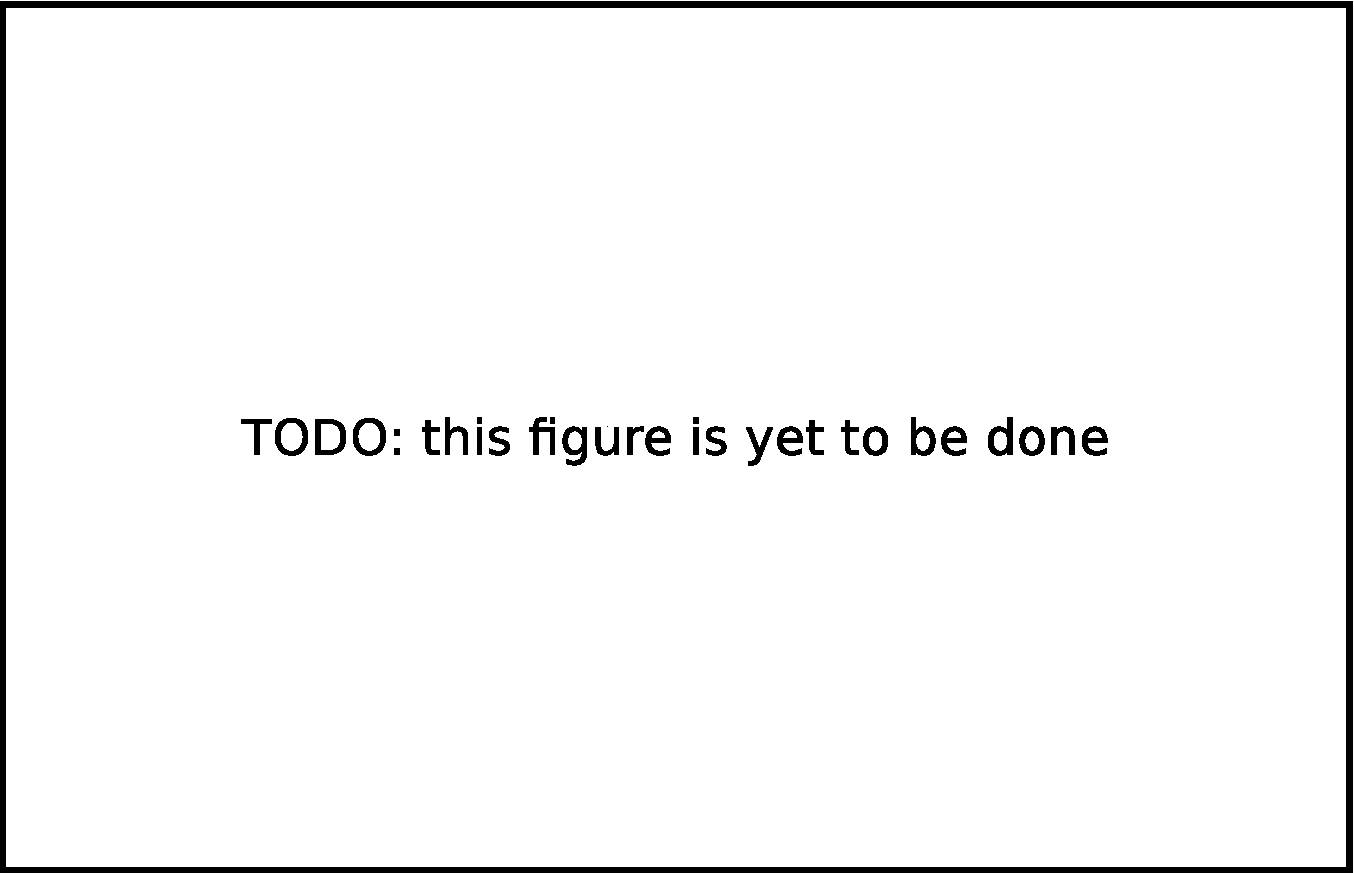
\includegraphics[scale=0.4]{fig/todo}
    \end{center}
    \caption{Class diagram of the \srccode{bna.bnlib.sampling} package.}
    \label{fig:sapling_package_class_diagram}
\end{figure}
\end{center}



\subsection{Producing a single sample}
Generally, a sample can be produced using many different sampling techniques (eg. direct sampling, weighted sampling, MCMC etc.) and the abstract class \srccode{SampleProducer} is a~common base class for such specific samplers. The class mainly keeps the specification of the distribution $P(\vars{X} \mid \vars{Y}, \vars{e})$ we want to sample and reference to the BN to be sampled.

List of noteworthy methods of the \srccode{SampleProducer} class:
\begin{itemize}
	\item \srccode{void determineSamplingOrder()}: A template method that computes list of variables whose values we need to keep track of during sampling and also determines the order of sampling, ie. specific sequence of variables. First of all, the order of sampling is computed using a linear time DFS-based topological sort algorithm~\cite{cormen_introduction_to_algorithms}. Then there is a hook \srccode{filterVariablesToSample(...)} by which the specific samplers (children of \srccode{SampleProducer}) can reduce the list of variables we need to take into account during sampling\,--\,this is useful for example in the case of weighted sampling. The final array of variables whose values need to be known/determined during sampling is stored in the instance variable \srccode{sampledVars}.
	\item \srccode{Variable[] filterVariablesToSample(Variable[] allVars)}: A hook of the template method \srccode{determineSamplingOrder()} described above. By default returns the argument, ie. no filtering.
	\item \srccode{void initializeSample(int[] assignment)}: Abstract method in which a concrete sampler may prepare the assignment of variables before the first sample is produced (needed in the MCMC sampling to set the evidence variables to given values). Specific values in the \srccode{assignment} array are instantiations of variables in \srccode{sampledVars} on the same indices.
	\item \srccode{double produceSample(int[] assignment)}: Abstract method to produce one sample and return its weight. The \srccode{assignment} array is filled with a concrete instantiation of respective variables of the array \srccode{SampleProducer.sampledVars}.
\end{itemize}


\subsubsection{Weighted sampling}
Weighted sampling is implemented by the class \srccode{WeightedSampleProducer}. As a subclass of \srccode{SampleProducer} it needs to define methods \srccode{initializeSample(...)}, \srccode{produceSample(...)} and also redefines the hook \srccode{filterVariablesToSample(...)} for optimization purposes.

List of noteworthy methods of the \srccode{SampleProducer} class:
\begin{itemize}
	\item \srccode{Variable[] filterVariablesToSample(Variable[] allVars)}: At this point the implementation weighted sampling takes advantage of the fact that, in order to produce relevant samples for determining the distribution $P(\vars{X} \mid \vars{Y}, \vars{e})$, we don't have to consider variables such that they are not in $\vars{X} \cup \vars{Y} \cup \vars{E}$ and also none of their descendants is in $\vars{X} \cup \vars{Y} \cup \vars{E}$. So, this method filters the given array of variables and preserves only those variables that don't satisfy the previously stated condition. This way weighted sampling can be accelerated for those queries in which a significant part of the BN doesn't need to be considered.
	\item \srccode{void initializeSample(int[] assignment)}: Empty method\,--\,during weighted sampling values of all variables are rewritten anyway, so there is no need to produce some initial instantiation.
	\item \srccode{double produceSample(int[] assignment)}: The weighted sampling is implemented as follows: We keep an array of \srccode{WeightedSamplingAction} objects. Each object is responsible for handling one variable of the \srccode{sampledVars} array (ie. the array of variables that need to be taken into account) so, one sample is produced by performing all the actions in a sequence.
	
	The associated action objects are different for evidence and for non-evidence variables.	For an evidence variable $E_i$ the associated \srccode{WeightedSamplingEvidenceAction} object extracts assignment of the variables $Parents(E_i)$ from the current sample (ie. current values in \srccode{assignment}) and determines the probability $P(E_i = e_i \mid parents(E_i))$ which will affect the weight of the sample.
	For a~non-evidence variable $X_i$ the associated \srccode{WeightedSamplingVariableAction} extracts assignment of the variables $Parents(X_i)$ from the current sample and then samples the variable $X_i$ from distribution $P(X_i \mid parents(X_i))$\,--\,sampling itself is actually implemented in the \srccode{Node} class. Finally, the value $x_i$ of variable $X_i$ is written to \srccode{assignment} on the right index.
\end{itemize}


\subsubsection{MCMC sampling}
\todo{MCMC resampling of variable $X$: the distribution $P(X \mid mb(X)$ is computed only by products of $P(x) P(children(X))$ instead of the whole Markov blanket}



\subsection{Answering a probabilistic query}
\srccode{QuerySampler}


\subsection{Multi-threaded sampling}
Class \srccode{QuerySamplerMultithreaded} is a multi-threaded variant of class \srccode{QuerySampler} and also aims to compute an approximation of distribution $P(\vars{X} \mid \vars{Y}, \vars{E} = \vars{e})$ through computing statistical properties of samples obtained from a given BN. We pass to the constructor of \srccode{QuerySamplerMultithreaded} a~\srccode{SampleProducer} object that provides samples on demand and the requested number of threads, the sampler instance creates and executes threads that perform sampling in parallel and finally their results are combined.

Speedup of the multi-threaded variant has been measured on multiple computers with different processors (see Table~\ref{tbl:sampling_multithread_speedup}). On a multi-processor system the speedup is significant, eg. on an 8 core system the speedup is according to measurements virtually 2 for two threads and about 3.8 for four threads.

\begin{table}[htb]
    \begin{center}
    \catcode`\-=12
    \begin{adjustwidth}{-0.85cm}{-0.75cm} % table wider than the text column would not be centered
    {\small
    % sprinkler network & weighted sampling
    \begin{subfigure}[b]{\linewidth}
        \begin{tabular}{|c|l|r|r|r|r|r|r|}
            % header
            \cline{3-8}
            \multicolumn{2}{c|}{} & \multicolumn{6}{c|}{\textbf{Number of threads}}\\
            \cline{3-8}
            \multicolumn{2}{c|}{} & 1 & 2 & 3 & 4 & 6 & 8\\ % #threads
            % my notebook Samsung 300V
            \hline
            \textbf{Intel i5-2450M} & \textbf{Samples/second}
                & 3.068e6 & 5.564e6 & 6.061e6 & 5.481e6 & 5.537e6 & 5.521e6\\
            \cline{2-8}
            \textbf{(2.5 GHz, 2 cores)} & \textbf{Speedup}
                & 1.00 & 1.81 & 1.98 & 1.79 & 1.80 & 1.80\\
            % merlin
            \hline \hline
            \textbf{2x Opteron 2387} & \textbf{Samples/second}
                & 2.429e6 & 4.765e6 & 6.911e6 & 9.160e6 & 10.803e6 & 11.672e6\\
            \cline{2-8}
            \textbf{(2.8 GHz, 4 cores)} & \textbf{Speedup}
                & 1.00 & 1.96 & 2.85 & 3.77 & 4.45 & 4.81\\
            % krok
            \hline \hline
            \textbf{Xeon E5-2640} & \textbf{Samples/second}
                & 1.977e6 & 4.106e6 & 5.867e6 & 7.307e6 & 9.190e6 & 10.739e6\\
            \cline{2-8}
            \textbf{(2.5 GHz, 6 cores)} & \textbf{Speedup}
                & 1.00 & 2.07 & 2.97 & 3.70 & 4.65 & 5.43\\
            % empty record
%            \hline \hline
%            \textbf{CPU id} & \textbf{Samples/second}
%                & sa1 & sa2 & sa3 & sa4 & sa6 & sa8\\
%            \cline{2-8}
%            \textbf{(cores info)} & \textbf{Speedup}
%                & 1.00 & sp2 & sp3 & sp4 & sp6 & sp8\\
            % final bottom line
            \hline
        \end{tabular}
        \caption{Weighted sampling of the classical \uv{sprinkler network} for query $P(Rain \mid WetGrass = true)$.}
    \end{subfigure}
    
    \bigskip
    % ICU network & weighted sampling
    \begin{subfigure}[b]{\linewidth}
        \begin{tabular}{|c|l|r|r|r|r|r|r|}
            % header
            \cline{3-8}
            \multicolumn{2}{c|}{} & \multicolumn{6}{c|}{\textbf{Number of threads}}\\
            \cline{3-8}
            \multicolumn{2}{c|}{} & 1 & 2 & 3 & 4 & 6 & 8\\ % #threads
            % my notebook Samsung 300V
            \hline
            \textbf{Intel i5-2450M} & \textbf{Samples/second}
                & 6.807e5 & 10.734e5 & 11.472e5 & 12.447e5 & 12.317e5 & 12.174e5\\
            \cline{2-8}
            \textbf{(2.5 GHz, 2 cores)} & \textbf{Speedup}
                & 1.00 & 1.57 & 1.69 & 1.83 & 1.81 & 1.79\\
            % merlin
            \hline \hline
            \textbf{2x Opteron 2387} & \textbf{Samples/second}
                & 4.880e5 & 9.786e5 & 13.718e5 & 18.237e5 & 26.643e5 & 32.237e5\\
            \cline{2-8}
            \textbf{(2.8 GHz, 4 cores)} & \textbf{Speedup}
                & 1.00 & 2.00 & 2.81 & 3.73 & 5.46 & 6.61\\
            % krok
            \hline \hline
            \textbf{Xeon E5-2640} & \textbf{Samples/second}
                & 4.384e5 & 9.398e5 & 13.775e5 & 17.493e5 & 23.337e5 & 27.361e5\\
            \cline{2-8}
            \textbf{(2.5 GHz, 6 cores)} & \textbf{Speedup}
                & 1.00 & 2.14 & 3.14 & 3.99 & 5.32 & 6.24\\
            % empty record
%            \hline \hline
%            \textbf{CPU id} & \textbf{Samples/second}
%                & sa1 & sa2 & sa3 & sa4 & sa6 & sa8\\
%            \cline{2-8}
%            \textbf{(cores info)} & \textbf{Speedup}
%                & 1.00 & sp2 & sp3 & sp4 & sp6 & sp8\\
            % final bottom line
            \hline
        \end{tabular}
        \caption{Weighted sampling of the \uv{ICU alarm network} for query $P(PVSAT \mid ECO2, SAO2 = high)$.}
    \end{subfigure}
    }
    \end{adjustwidth}
    \caption{Benchmark results of multi-threaded sampling speedup on various processors. Each value $samples/second$ was computed as follows: 20 million samples divided by the median computation time of sampling from total of 25 runs.
    \ignore{Median was used because sometimes the computation was really slow (typically the very first sampling)}\\
    The first machine is my notebook and the others are student servers merlin and krok at the university.
    }
    \label{tbl:sampling_multithread_speedup}
    \end{center}
\end{table}

\medskip
During implementation there have been some difficulties regarding thread-safety and sharing of resources among threads. The main problem turned out to be that an instance of \srccode{java.util.Random} (further just \srccode{Random}) cannot be shared among multiple threads because the key method \srccode{Random.next(int bits)} for generating pseudorandom bits is synchronized and sharing of a \srccode{Random} instance among $n$ threads degrades computation time to virtually running the sampling $n$-times sequentially. The problem is easily solved by using \srccode{java.util.concurrent.ThreadLocalRandom} class that provides the caller with a~thread-local instance of \srccode{Random} on demand. Still, generating of random data itself is the bottleneck of sampling.

Also, we cannot save time by storing references to dynamically allocated objects (eg. arrays) holding intermediate results if theses objects aren't read only, since concurrent threads would rewrite each others values. Fortunately, it turns out that frequent memory allocation for such intermediate results in Java doesn't introduce a bottleneck.







\section{Structure learning}
\todo{Could use Warshall algorithm to determine which edges can be added/deleted/reversed without the need to try such modification and consequently check for acyclicity}






\section{User interface}





















\chapter{Selected applications}
This chapter will present collection of selected applications suitable for Bayesian network learning. We will always examine the problem itself, reason why it is interesting, approach to its solution and the achieved results. At the time of writing the term project, candidate applications are the ones described in the rest of this chapter. Extent of this chapter is expected to be 10-15 pages.

\section{ICU alarm network (general model learning)}
The \term{ICU alarm network}\footnote{The ICU alarm network is, among others, freely available at The Hebrew University of Jerusalem \ignore{\url{http://www.bnlearn.com/bnrepository/}}\url{http://www.cs.huji.ac.il/site/labs/compbio/Repository/networks.html}.} (ICU stands for \term{Intensive care unit}) serves in the world of Bayesian networks as a benchmark for parameter and structure learning algorithms. The network itself has been hand-constructed and tuned in cooperation with the ICU personal. There are two types of goals: (a)~we attempt to learn parameters for a known structure, (b)~we attempt to learn both structure and parameters. Because the network is freely available, the usual course of action is to create an artificial dataset by sampling the original network, then performing the learning process and finally evaluating the obtained result by comparison with the original ICU network. 


\section{Crime prediction (knowledge discovery)}
We are given a dataset\footnote{The dataset \emph{Communities and crime} is available at \url{http://archive.ics.uci.edu/ml/datasets/Communities+and+Crime}.} containing records for various communities across the United States. A single record contains features such as racial representation, income, family completeness, housing etc. and the number of violent crimes. The goal is to find a structure of a BN that will hopefully provide us with better insight into causal dependencies between features and that can potentially help us identify the root causes of crime.

Similar task has been previously inspected as a school project for the "Knowledge Discovery in Databases (2012/2013)" class at BUT FIT by me and Petr Beňas. We learned that transforming each continuous value to membership degrees to three fuzzy sets (low, medium, high) preserves variance of the data which might be useful because the data could be discretized and the learning process would be relatively simple. Knowledge discovery techniques used in the project did not include any probabilistic model.


\section{Spam filtering (document classification)}
For a given set of training e-mails, we need to preprocess the data and extract relevant features (keywords, sender domain, font color, numbers and currency symbols etc.) to form a feature vector. Some of the features may be hand-crafted, other might be automatically selected, for example by the highest mutual information between a feature $X_i$ and the class variable~$C$. Then we may learn (1) a Naïve Bayesian model, (2) an extension of the naive model which also allows for a limited degree of dependencies between features. Finally, we can analyze the increase in accuracy (if any) of the more complex and more expressive model.

The usefulness of Naïve Bayesian model for spam classification has been studied in~\cite{heckerman98_spam}.

\begin{comment}
\todo{
\begin{itemize}
	\item Medical diagnosis (from a big dataset of patient records)\,--\,structure and CPDs.
	\item Pedigrees (BUT structure is known).
	\item protein networks (how a protein influences another protein)\,--\,lecture "Learning General Graphs: Heuristic Search", dataset at \url{http://www.causality.inf.ethz.ch/repository.php}
\end{itemize}
}
\end{comment}








\chapter{Conclusion}
During the term project I focused on studying the theory of Bayesian networks, mainly from the books~\cite{pgm,russell_norvig_ed2}. As a supporting material I also attended an on-line course called Probabilistic Graphical Models at \url{http://www.coursera.org} taught by professor Daphne Koller at Stanford University.

I explained the fundamentals of Bayesian networks, described various methods of inference (exact, stochastic and message passing) and methods of model learning. I also focused on explaining strong points and limitations throughout this thesis. All techniques have been studied and presented in such a detail that is needed in order to successfully implement them and to understand their limitations.

\medskip

In the summer semester I am going to study the selected application cases in depth and provide a program realization. At first, I am going to attempt to reproduce results achieved by other authors and then possibly apply the presented techniques to other problems or to achieve better results than have been presented. If needed, I will also study specific variants of model learning (especially from~\cite{heckerman96} and~\cite{buntine94}) and stochastic inference (especially from~\cite{neal93}). Furthermore, the book~\cite{pgm} provides an extensive list of relevant literature for every topic presented in this thesis. % SP
%=========================================================================
%begin-of-inserted-footer











% Pouzita literatura
  % ----------------------------------------------
\ifczech
  \bibliographystyle{czechiso}
\else 
  \bibliographystyle{plain}
%  \bibliographystyle{alpha}
\fi
  \begin{flushleft}
  \bibliography{literatura} % viz. literatura.bib
  \end{flushleft}
  \appendix
  
  \chapter{Notation overview}\label{ch:appendix_notation}
This chapter presents listing of the mathematical notation used in this thesis:

\bigskip
\begin{tabular}{ll}
	$X$ & Capital letter denotes a random variable.\\
	&\\
	$x$ & Lowercase letter denotes a concrete instantiation of the variable $X$.\\
	&\\
	$\vars{X}$ & Capital bold letter denotes a set of random variables.\\
	&\\
	$\vars{x}$ & Lowercase bold letter denotes an instantiation of all variables in the set $\vars{X}$.\\
	&\\
	$val(\vars{X})$ & Set of all possible instantiations of variables $\vars{X}$.\\
	&\\
	$Parents(X)$ & Set of parent variables of variable $X$ in a Bayesian network.\\
	&\\
	$parents(X)$ & Instantiation of parent variables of variable $X$ in a Bayesian network.\\
	&\\
	$Children(X)$ & Set of child variables of variable $X$ in a Bayesian network.\\
	&\\
	$children(X)$ & Instantiation of child variables of variable $X$ in a Bayesian network.\\
	&\\
	$N_x$ & Number of samples of a dataset for which variable $X$ has the value $x$.\\
	&\\
	$N_{x,\vars{pa}}$ & Number of samples of a dataset for which $X$ has the value $x$ and variables\\
	                  & $Parents(X)$ have the value $\vars{pa}$.\\
	&\\
	$\sum_\vars{X} (\dots)$ & Summation over instantiations $\vars{x}$ of the variables $\vars{X}$.\\
	&\\
	$P(\vars{X})$ & Probability distribution over variables $\vars{X}$.\\
	&\\
	$P(\vars{x})$ & Probability of variables $\vars{X}$ having the concrete instantiation $\vars{x}$.\\
\end{tabular}










\chapter{CD Content}\label{ch:appendix_cd_content}
Content of the enclosed CD is organized into the following directories:
\begin{itemize}
    \item \srccode{1-benchmarks/}: Network \srccode{.net} files, datasets and measurements related to the first practical application.
    \item \srccode{2-crime/}: Vector images of the final three networks that resulted from the analysis of criminality. Also contains the original dataset, its discretized version, networks learnt during the feature elimination process and records of analysis of the crime impact factor.
    \item \srccode{3-spam/}: Datasets (the original dataset, its discretized version, train and test sets for holdout testing and for 5-fold cross-validation). Also contains measurement records and figures.
    \item \srccode{program/}: Program source codes compilable using the \emph{ant} build tool and also runnable compiled version in \srccode{program/bin-precompiled}.
    \item \srccode{text/}:  {\LaTeX} sources of this thesis, including all figures.
\end{itemize} 





\chapter{Crime analysis\,--\,final networks}\label{ch:appendix_crime_net}
This chapter contains the three networks that are result of the crime analysis performed in Section~\ref{ch:practical_crime}. Because of their size, each network is on its own A3 page. If you have trouble reading variable names in the printed version please see the electronic version of this thesis or the original figures on the encolsed CD within the directory \srccode{2-crime/final networks/}.


\begin{hugepage}
\pdfpagewidth=2\pdfpagewidth
\begin{figure}[h]
    \centering
    \vspace*{-2.5cm}
    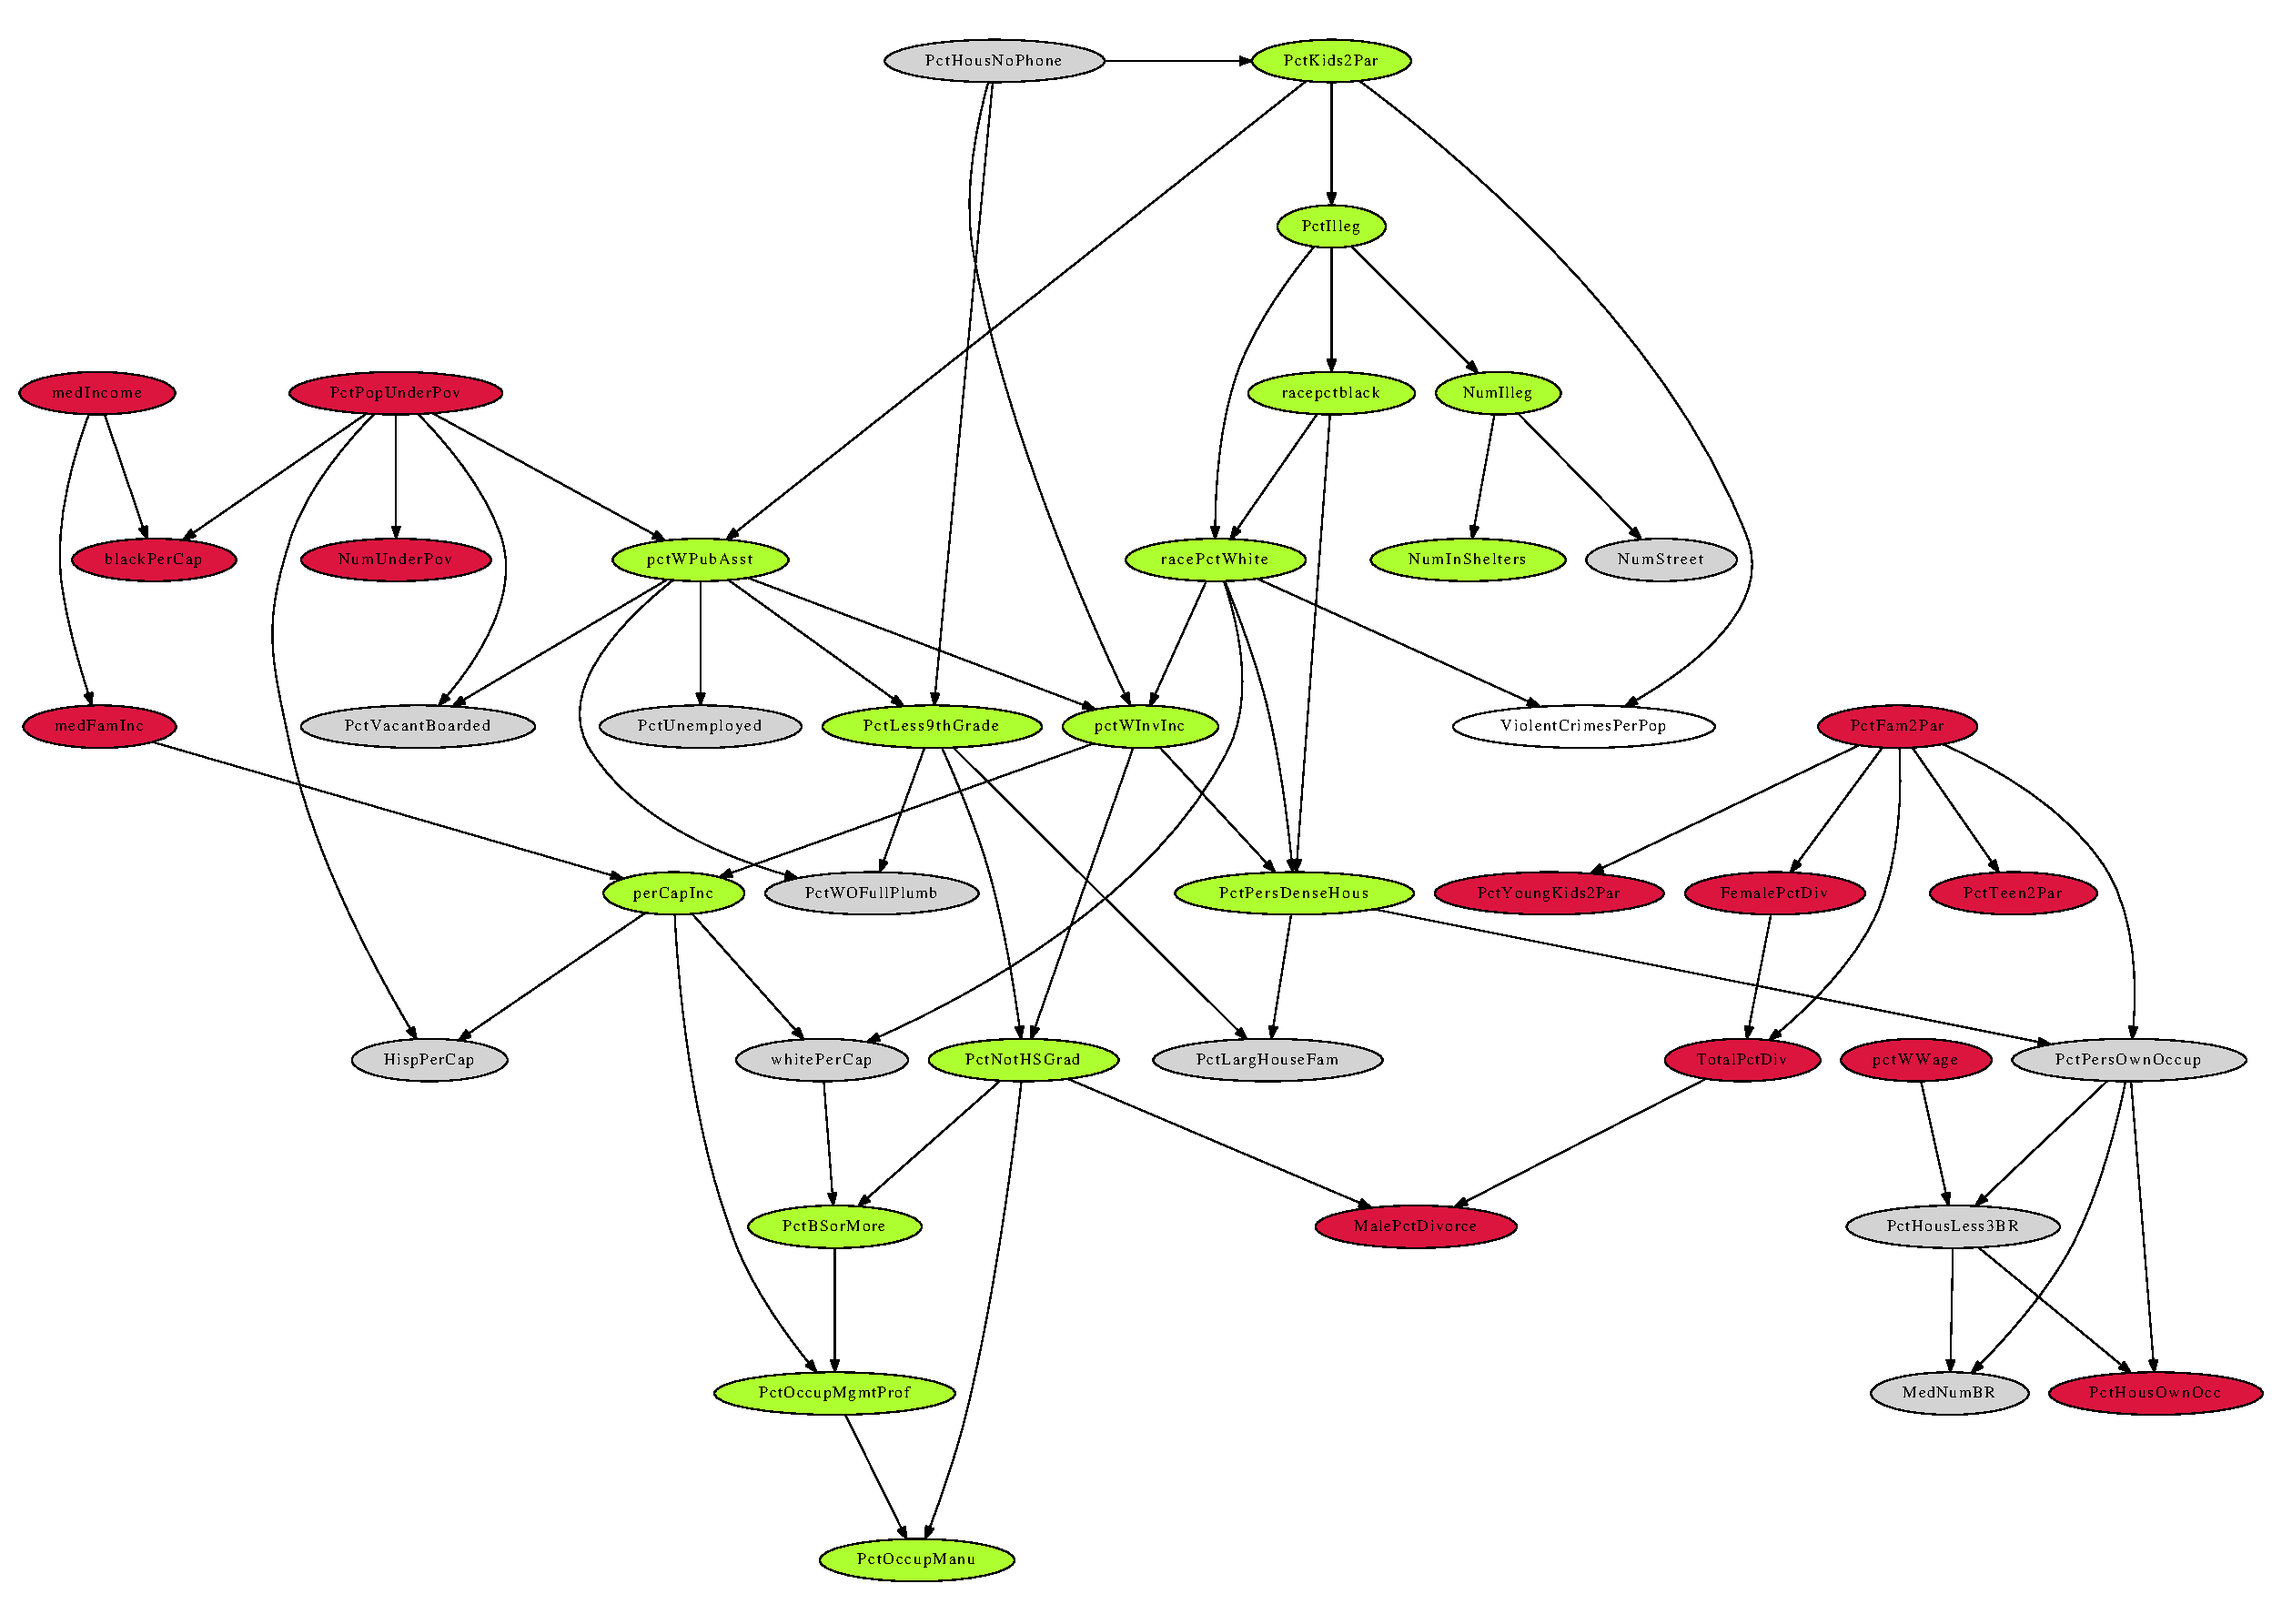
\includegraphics[scale=0.834]{fig/top-40_intersection_tolerance-1}
    \caption{Bayesian network for crime containing top 40 attributes with the highest crime impact factor.
    \\Legend: Green variables influence the $ViolentCrimesPerPop$ the same way as in the network with all 100 features. Influence of red variables is significantly different and therefore these variables shouldn't be considered.}
    \label{fig:crime_net_top40}
\end{figure}
\end{hugepage}

\begin{hugepage}
\pdfpagewidth=2\pdfpagewidth
\begin{figure}[h]
    \centering
    \vspace*{-2.5cm}
    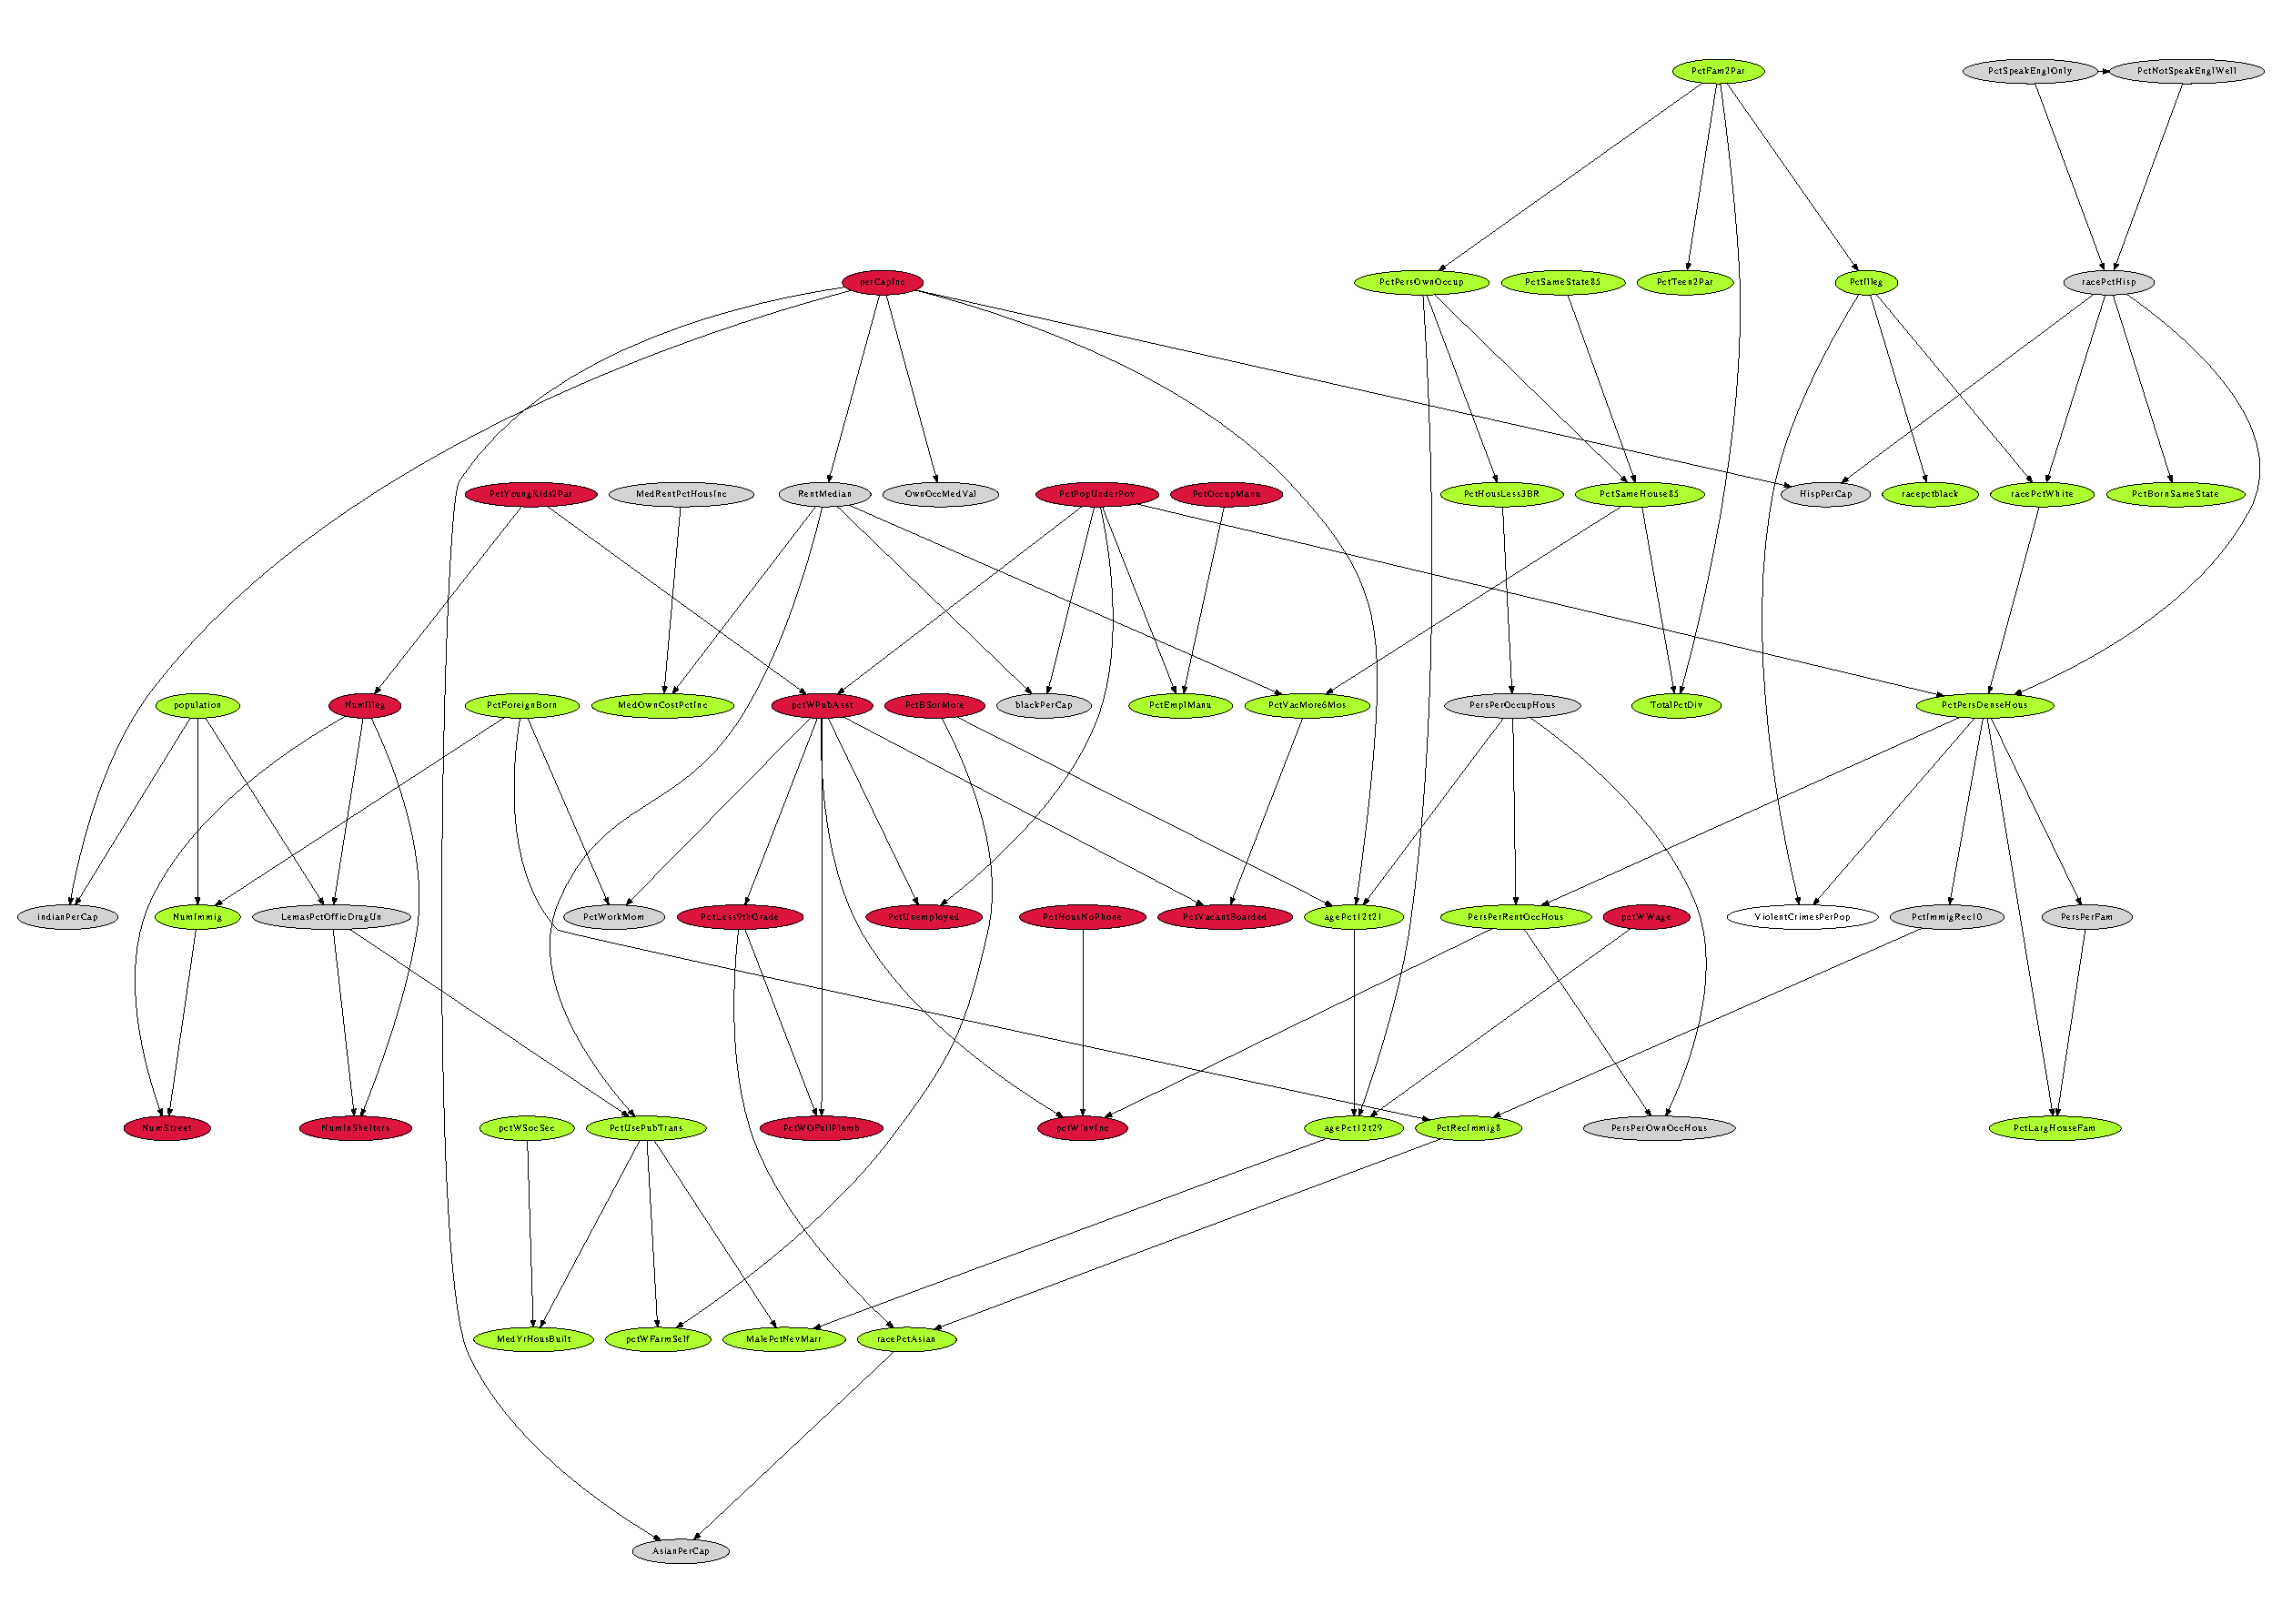
\includegraphics[scale=0.83]{fig/round-3_intersection_tolerance-1}
    \caption{Final Bayesian network for crime after three rounds of iterative elimination of similar variables.
    \\Legend: Green variables influence the $ViolentCrimesPerPop$ the same way as in the network with all 100 features. Influence of red variables is significantly different and therefore these variables shouldn't be considered.}
    \label{fig:crime_net_round3}
\end{figure}
\end{hugepage}

\begin{hugepage}
\pdfpagewidth=2\pdfpagewidth
\begin{figure}[h]
    \centering
    \vspace*{-2.5cm}
    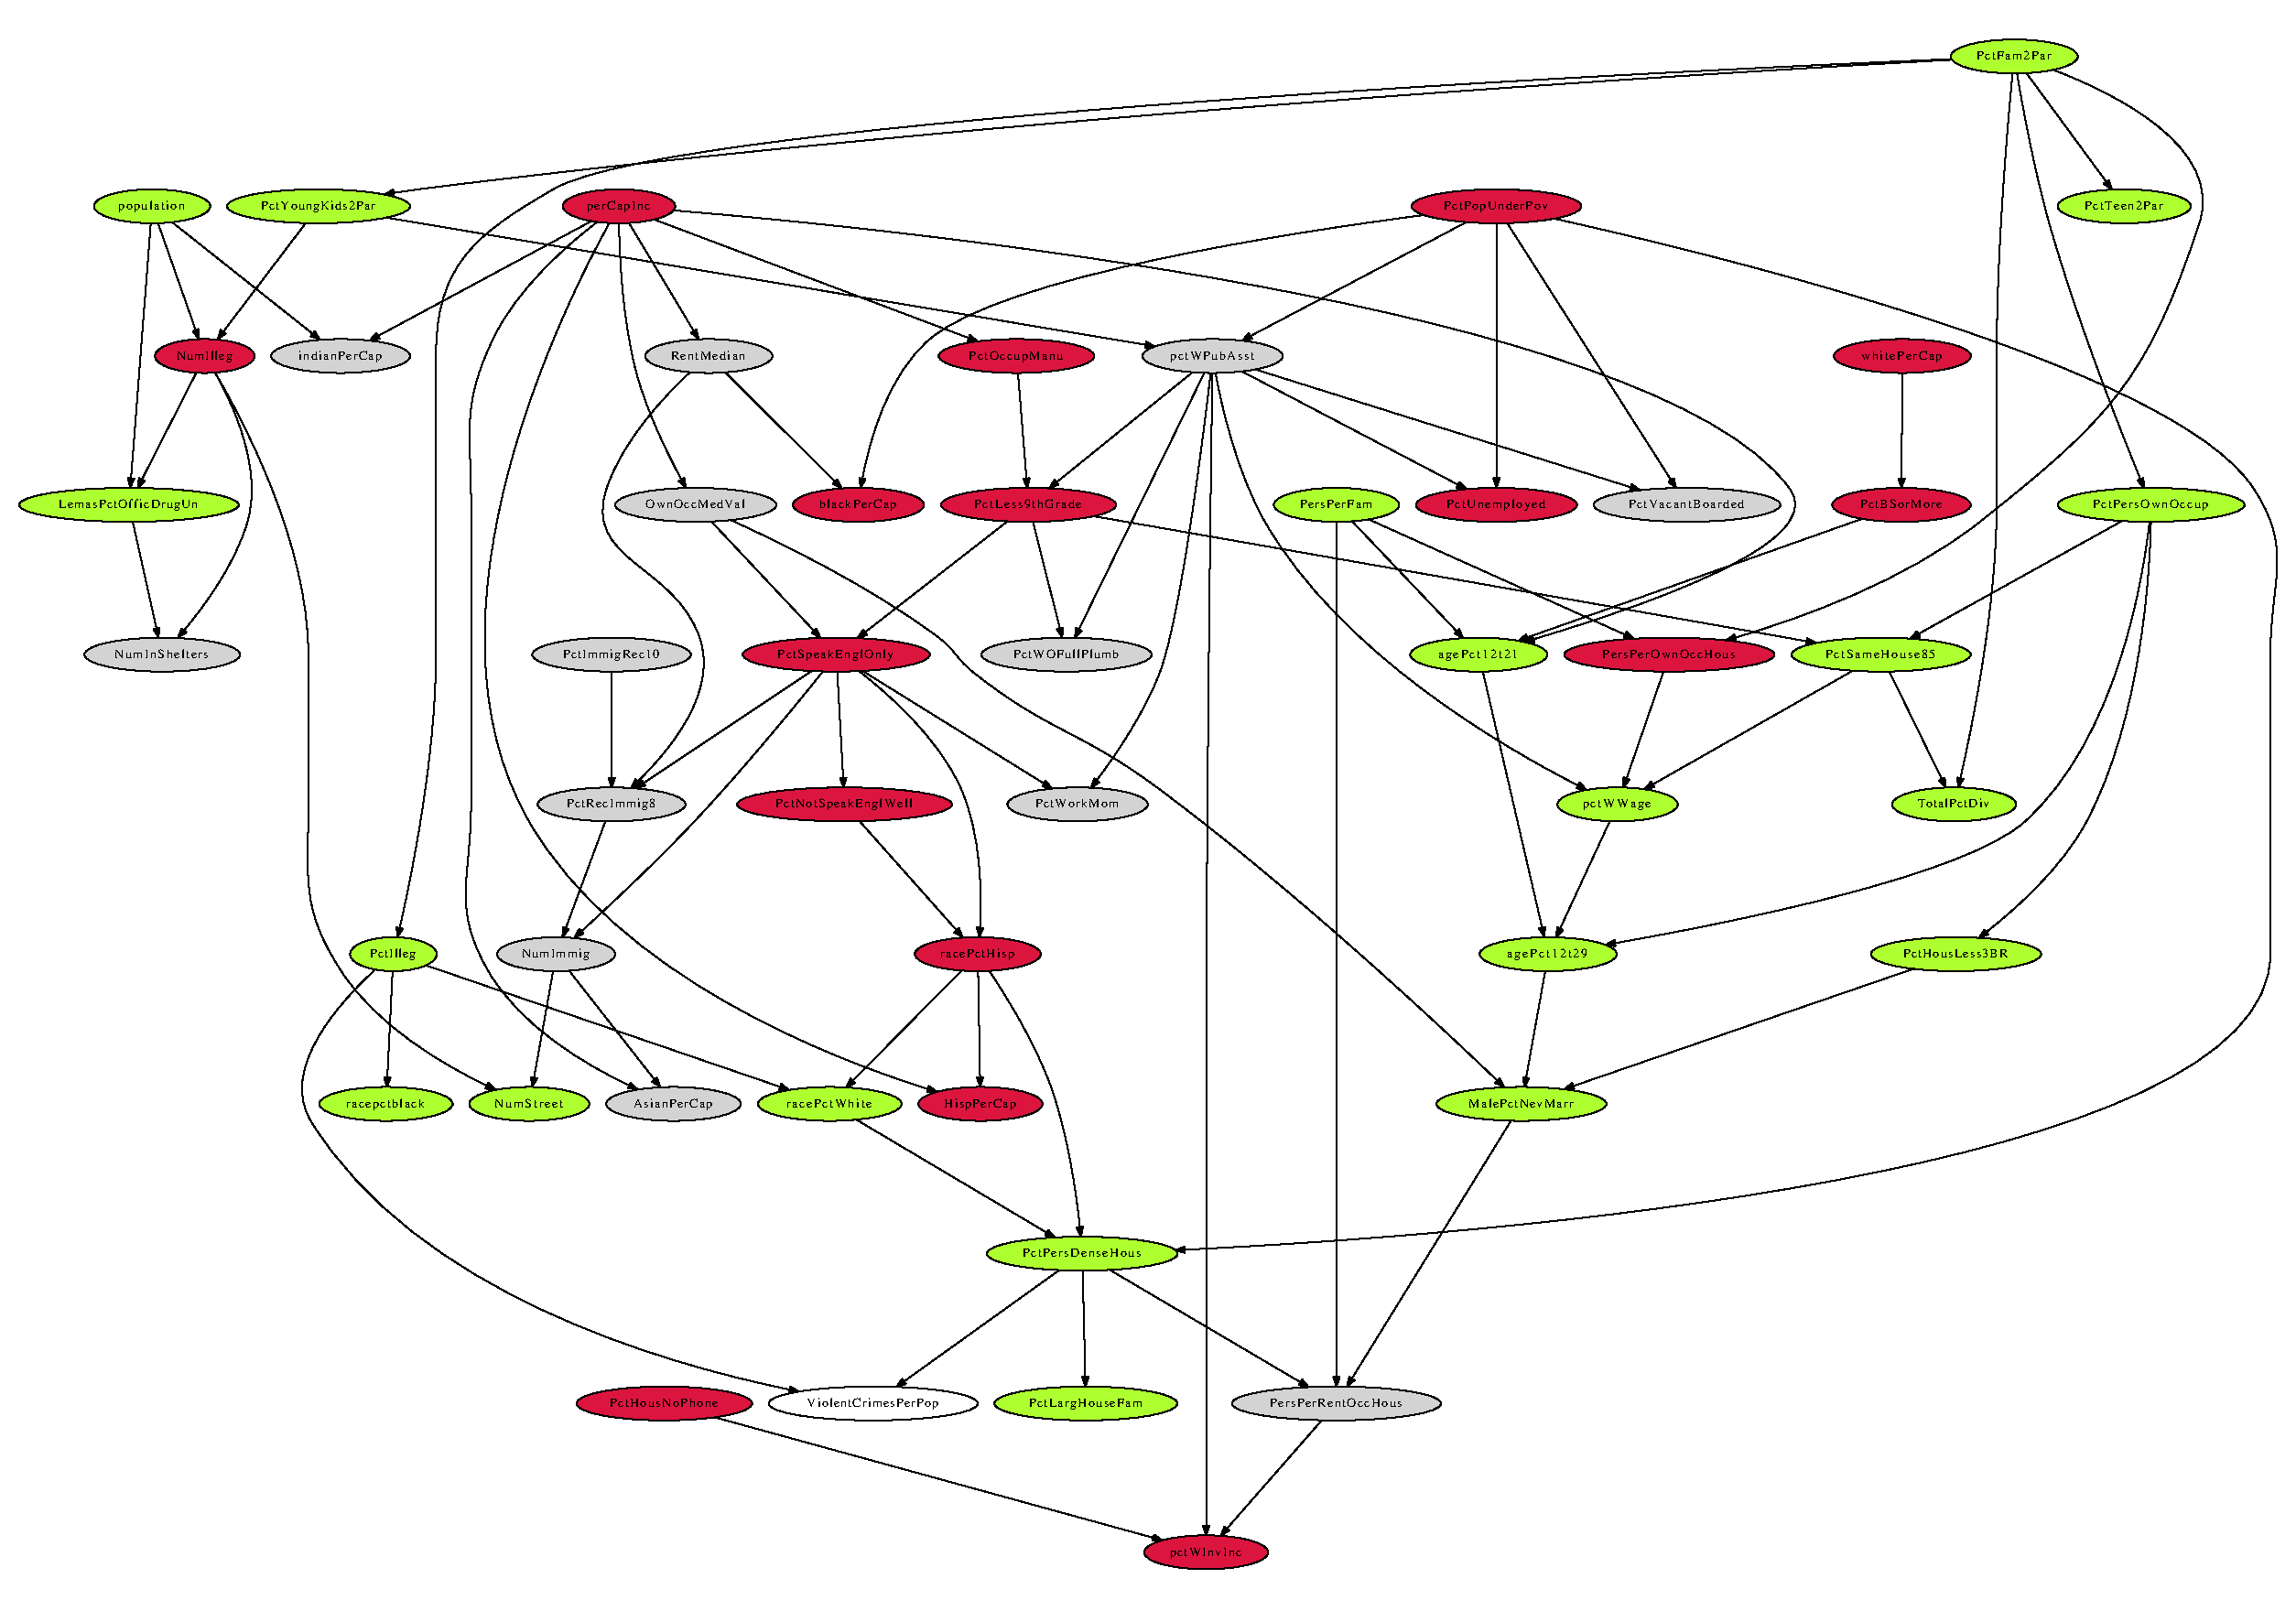
\includegraphics[scale=0.83]{fig/round-4_intersection_tolerance-1}
    \caption{Final Bayesian network for crime after three rounds of iterative elimination of similar variables and additional removal of variables whose crime impact factor is less than 0.07.
    \\Legend: Green variables influence the $ViolentCrimesPerPop$ the same way as in the network with all 100 features. Influence of red variables is significantly different and therefore these variables shouldn't be considered.}
    \label{fig:crime_net_round4}
\end{figure}
\end{hugepage}


 % viz. prilohy.tex
\end{document}
